\section{Application performance}
\label{sec:eval:apps}

\makeatletter
\def\input@path{{eval/apps/}}
\makeatother
\graphicspath{{eval/apps/figures/}}



\begin{table}[t!b!]
\subsection{End-to-end application performance}
\label{sec:eval:perf:apps}


\begin{table}[t!b!]
\subsection{End-to-end application performance}
\label{sec:eval:perf:apps}


\begin{table}[t!b!]
\subsection{End-to-end application performance}
\label{sec:eval:perf:apps}


\begin{table}[t!b!]
\input{tables/apps}
\caption{Application benchmark execution times in a (1) native Linux process, (2) a process inside a KVM virtual machine, (3) a \graphene{} \picoproc{} with the SECCOMP filter ({\bf +SC}) and reference monitor ({\bf +RM}). }
\label{tab:graphene:apps}
\end{table}



Table~\ref{tab:graphene:apps} lists 
execution time of our {\em unmodified} 
application benchmarks (detailed in \S\ref{sec:eval:graphene}).
All applications create multiple processes,
except for \lighttpd{}, which only creates multiple threads.
Each data point is the average of at least six runs, 
and 95\% confidence intervals are listed in the table.

We exercise  {\tt \gcc{}}/{\tt make}
with inputs of varying sizes:
%the pbzip2 compression utility (v1.1.6, 4 KLoC),
%the ogg sound encoder (v1.0.1, 5 KLoC),
%GNU {\tt make} (v3.82, \fixmedp{XX} KLoC)
bzip2 (v1.0.6, 5KLoC, 13 files),
\graphene{}'s {\tt libLinux} (31 KLoC, 78 files)
and \gcc{} (v3.5.0, 551 KLoC, collected as a single source file). 
We benchmark Apache (4 preforked workers) and \lighttpd{} (4 threads) with 
\ab{},
which issues 25, 50, and 100 concurrent requests
to download a 100 byte file 50,000 times.

We exercised \busy{} with 
300 iterations of the Unixbench benchmark~\cite{unixbench}, as well as 
300 iterations of a simple shell script benchmark that runs 6 common shell script commands
({\tt cp}, {\tt rm}, {\tt ls}, {\tt cat}, {\tt date}, and {\tt echo}).

Compilation workloads incur overheads ranging from 5--30\%.
%All compilation workloads have minimal overheads compared to native when executed sequentially;
Parallel compilation on both \graphene{} and Linux yields comparable  speedups  over sequential,
but the percent overhead increases for parallel \graphene{}.
For instance, {\tt make -j4 libLinux} speeds up 3.7\x{} on Linux and 3.4$\times$ on \graphene{}.
The compilation overheads are primarily from the reference monitor---nearly all for bzip2 and gcc, and half for {\tt libLinux}.
%Nearly all of the overhead from the bzip2 and gcc compilations are from the reference monitor; about half of the overheads of {\tt libLinux} compile 
%are the reference monitor and half are \graphene{} itself.
In the case of both \busy{} workloads, the key bottleneck is the {\tt fork} system call.
Profiling indicates that half of the time in {\tt libLinux} is spent on {\tt fork} in both benchmarks.
The trend is exacerbated in Unixbench, which creates all of the processes at the beginning and
waits for them all to complete; because \graphene{} cannot create children as quickly as native, this leads to 
load imbalance throughout the rest of the benchmark.  

With the reference monitor disabled,  \lighttpd{} has equivalent throughput to a native Linux process;
as discussed in the next subsection, these overheads come from checking paths in the monitor.
The Apache web server loses about half of its throughput relative to \lighttpd{} on \graphene{}.
The primary bottleneck in Apache relative to \lighttpd{} is System V semaphores,
%, which account for about 
%one third of the additional time spent in {\tt libLinux}
%relative to \light{}, 
and the remaining overheads are attributable to more time spent waiting for input.
The overheads for both \lighttpd{} and Apache on KVM are primarily attributable
to bridged networking.


One deployment model for SGX is to host network services
on an untrusted cloud provider's hardware.
%To measure this case, 
We measure three widely-used Linux web servers, including {\bf Lighttpd}~\cite{lighttpd} (v1.4.35), {\bf Apache}~\cite{apache} (v2.4.18), and {\bf NGINX}~\cite{nginx} (v1.10).
%, to evaluate the performance of server-type workloads in \graphenesgx{}.
%These applications are all sophisticated, non-trivial workloads, and are constantly being used for commercial purposes.
%We test these applications to evaluating significantly different execution patterns, to benchmark the performance of \graphenesgx{} under each circumstances.
%Also, we do not explicitly configure these servers to secure their payloads using the HTTPS protocol.\fixme{if have time, maybe try again with HTTPS}
For each workload, we use ApacheBench~\cite{apachebench} to download the web pages on a separate machine.
%\edit{over Gigabit LAN}. %\fixmedp{more specific?}
%across a high-speed \fixmedp{Can you say
%more specifically the specs, like 10 GBps or whatever; also, if this is the same vlan, I might just describe this as being on a LAN, minimizing interference} University network.
The concurrency of ApacheBench is gradually increased during the experiment, to test the both the per-request latency and the overall throughput of the server.
Figure~\ref{fig:server-throughput-latency} shows the throughput versus latency of these server applications
in \graphenesgx{}, \graphene{} and Linux. 
Each workload is discussed below.




% Put figures at the front
\begin{figure*}[t!]
\centering

\begin{minipage}{.45\textwidth}
\centering
\footnotesize
\vspace{6pt}
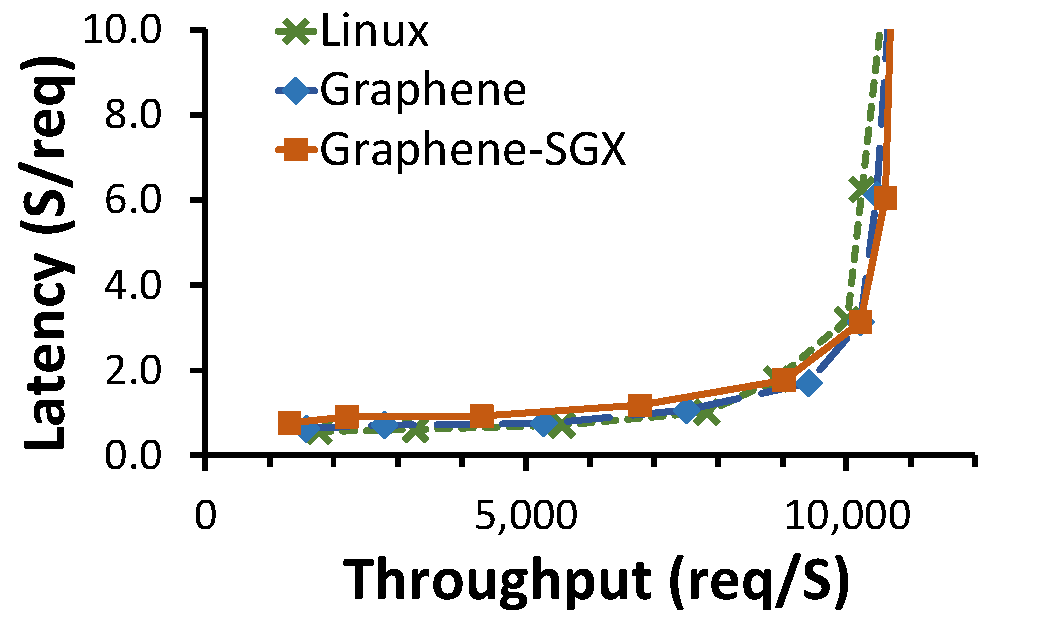
\includegraphics[width=\linewidth]{sgx/lighttpd-throughput-latency}\\
\vspace{3pt}
{\bf (a) Lighttpd (25 threads)}
\vspace{6pt}
\end{minipage}
\begin{minipage}{.45\textwidth}
\centering
\footnotesize
\vspace{6pt}
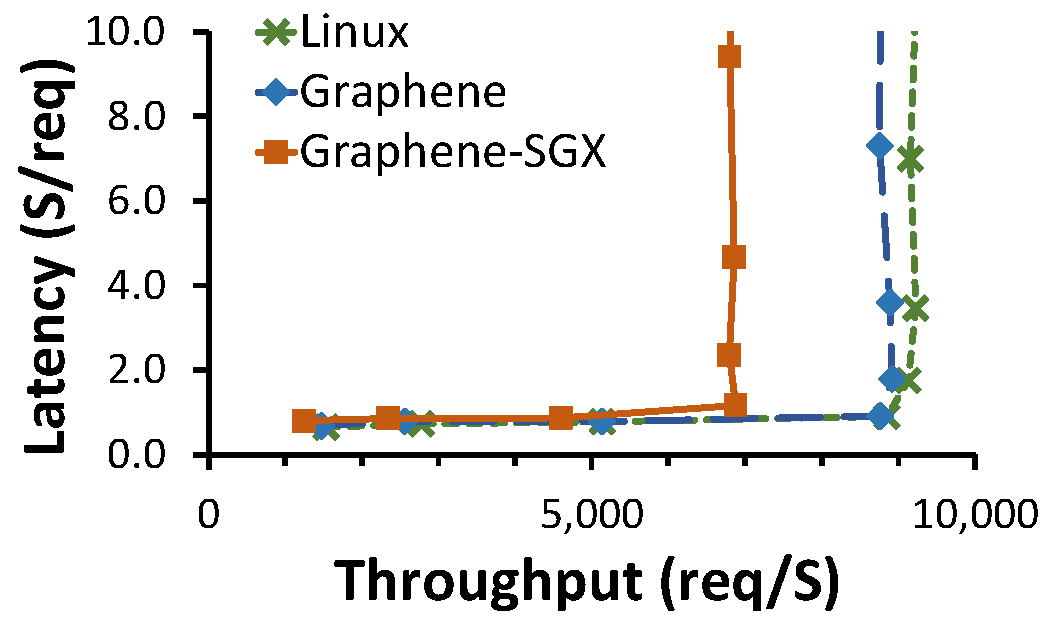
\includegraphics[width=\linewidth]{sgx/apache-throughput-latency}\\
\vspace{3pt}
{\bf (b) Apache (5 processes)}
\vspace{6pt}
\end{minipage}
\begin{minipage}{.45\textwidth}
\centering
\footnotesize
\vspace{6pt}
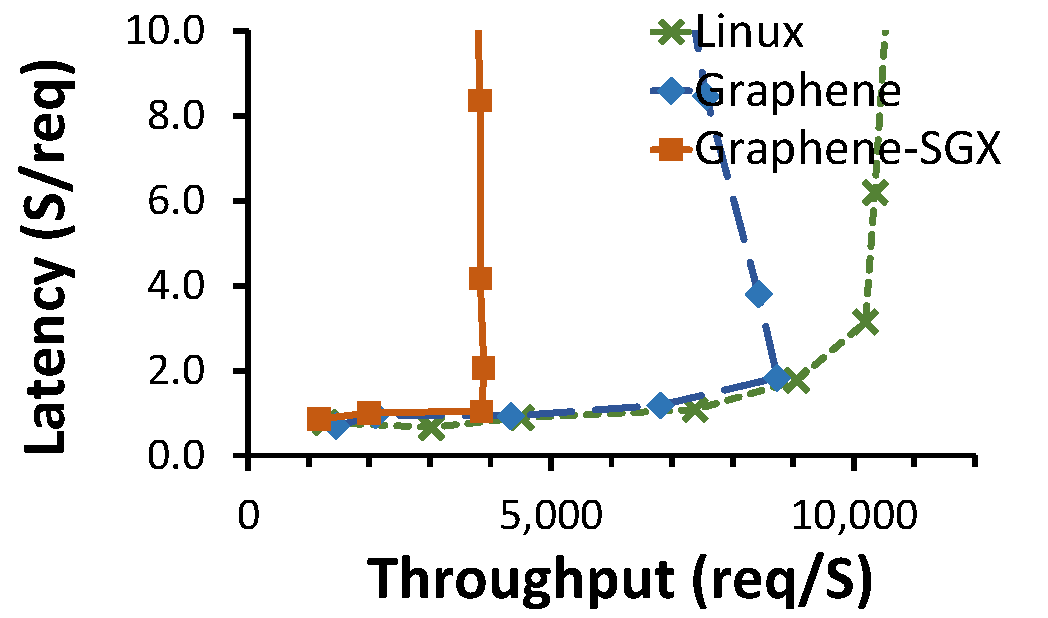
\includegraphics[width=\linewidth]{sgx/nginx-throughput-latency}\\
\vspace{3pt}
{\bf (c) NGINX (event-driven)}
\vspace{6pt}
\end{minipage}

\caption{Throughput versus latency of web server workloads, including Lighttpd, Apache, and NGINX, on native Linux, \graphene{}, and \graphenesgx{}.
We use an ApacheBench client to gradually increase load, and plot
throughput versus latency at each point.  Lower and further right
is better.
%\fixmedp{RB: Add another sentence or two to explain what the experiment is and how to interpret} }
}
\label{fig:server-throughput-latency}
\end{figure*}


{\bf Lighttpd}~\cite{lighttpd} is a web server designed to be light-weight, yet robust enough for commercial uses. 
Lighttpd is multi-threaded; we test with 25 threads to process HTTP requests. 
By default, Lighttpd uses the \syscall{epoll\_wait} system call to poll listening sockets.
At peak throughput and load,  both \graphene{} and \graphenesgx{} have marginal overhead on either latency or throughput of the Lighttpd server.
The overheads of \graphene{} are more apparent when the system
is more lightly loaded, at 
%When Lighttpd is not overloaded, \graphenesgx{} causes 
15--35\% higher response time, or 13--26\% lower throughput. 
Without SGX, \graphene{} induces 
11--15\% higher latency or 13-17\% lower throughput over Linux;
the remaining overheads are attributable to SGX---either hardware or our OS shield.
%platform adaptation layer (PAL) code.

%\fixmedp{Some more detailed analysis would be nice.}
%Only part of this overhead is contributed by the library OS implementation, since using \graphene{} without \sgx{} causes only 

%\fixmedp{Why did you comment this out?  Let's discuss: Does it really make sense to have two points at the same  x-axis value?  Perhaps the axes should be inverted?  I'm not really sure about the methodology, but something about the line doubling back on itself seems wrong.  Maybe you want to separate these and show throughput vs. load, and a CDF of latencies?}


{\bf Apache}~\cite{apache} is one of the most popular production web servers. We test Apache using 5 preforked worker processes to service HTTP requests,
in order to 
to evaluate the efficiency of \graphenesgx{} across enclaves.
%n server, 
%In the experiment, the Apache server creates 5 preforked processes which coordinate on processing HTTP requests.
This application uses IPC extensively---the preforked processes of a server use a System V semaphore to synchronize on each connection.
%When receiving a connection, the preforked processes of Apache will coordinate among themselves using the system V IPC semaphores.
Regardless of the workload, the response time on \graphenesgx{} is 12--35\% higher than Linux, due to the overhead of coordination across enclaves over encrypted RPC streams.
The peak throughput achieved by Apache running in \graphenesgx{} is 26\% lower than running in Linux.
In this workload, most of the overheads are SGX-specific, such as exiting enclaves when accessing the RPC, as non-SGX Graphene
has only 2--8\% overhead compared to Linux.

%The enclave restriction \fixmedp{Huh?} is the main contributor to this overhead, as \graphene{} generally only causes 2--8\% overhead.

%\fixmedp{Check the lightttp graph; the lines are right on top of each other, and dont' look 22\% apart to me.  Some of this may be the scale of the y axis}

{\bf NGINX}~\cite{nginx} is a relatively new web server designed for high programmability, for as a building block to implement different services.
Unlike the other two web servers, NGINX is event-driven and mostly configured as single-threaded.
%When running as a simple HTTP server, NGINX uses an event-driven model instead of multi-threading/multi-processing to handle incoming requests.
\graphenesgx{} currently only supports synchronous I/O at the enclave boundary,
and so, under load, it cannot as effectively overlap I/O and computation
as other systems that have batched and asynchronous system calls.
%Asynchronous system calls and events in general are less mature features of
%\graphenesgx{}, and, 
Once sufficiently loaded, NGINX on both \graphene{} and \graphenesgx{} 
performs worse than in a  Linux process. % once sufficiently loaded.
%We observe that both \graphene{} and \graphenesgx{} tend to perform poorly in an event-driven server.
The peak throughput of \graphenesgx{} is 1.5$\times$ lower than Linux;
without SGX, Graphene only reaches 79\% of Linux's peak throughput.
%\fixmedp{Maybe shout out to eleos, or cite other work}
We expect that using tools like Eleos~\cite{orenbach17eleos} to reduce exits
would help this workload; in future work, we will improve
asynchronous I/O in \graphenesgx{}.

%\graphenesgx{} causes 17--90\% more response time when the server is not overloaded,
%but up to 1.5$\times$ at the peak throughput.
%If we compare the peak throughput with native Linux, \graphenesgx{} is 70\% less.
%\graphene{} also suffers the same performance pattern, as the throughput drops dramatically after reaching 79\% of the peak throughput of NGINX in Linux.
%The reason of the slowdown is that the host interface of \graphene{} and \graphenesgx{} only supports synchronous IO, so implementing asynchronous IO will be less efficient. This limitation is a trade-off to the portability of \graphene{}.
%\fixmedp{Didn't get the portability point; please spell out what you meant, if important}


\begin{figure}[t!]
\centering
\footnotesize
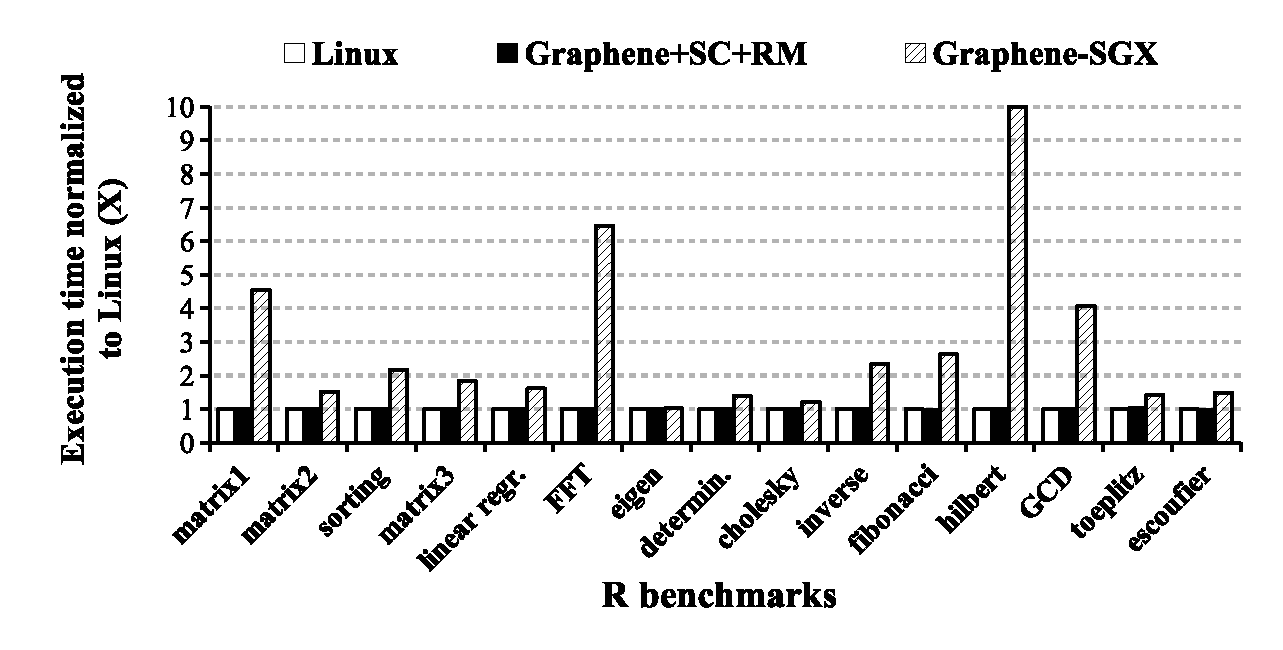
\includegraphics[width=38em]{r-overhead}\\
\caption{Performance overhead on desktop applications, including latency of R, execution time of GCC compilation, download time with CURL. The evaluation compares native Linux, \graphene{}, and \graphenesgx{}.} %{\bf Enclave creation time is deducted from the GCC execution time.}}
\label{fig:eval:r-overheads}
\end{figure}


\begin{figure}[t!]
\centering
\footnotesize
\begin{minipage}{.49\textwidth}
\centering
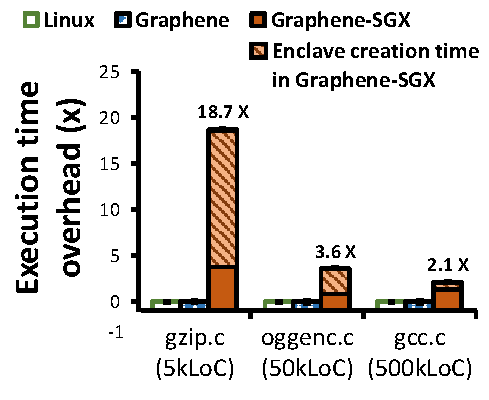
\includegraphics[width=20em]{sgx/gcc-overhead}\\
\vspace{3pt}
{\bf (b) GCC}
\end{minipage}
\begin{minipage}{.49\textwidth}
\centering
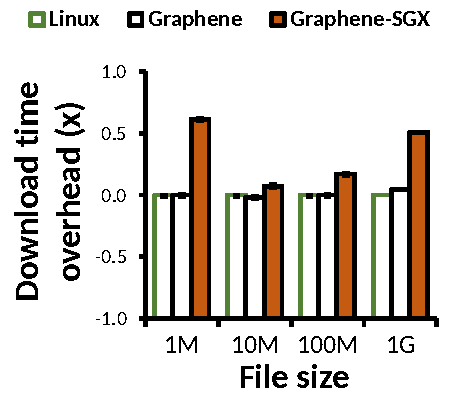
\includegraphics[width=20em]{sgx/curl-overhead}\\
\vspace{3pt}
{\bf (c) CURL}
\end{minipage}
\caption{Performance overhead on desktop applications, including latency of R, execution time of GCC compilation, download time with CURL. The evaluation compares native Linux, \graphene{}, and \graphenesgx{}.} %{\bf Enclave creation time is deducted from the GCC execution time.}}
\label{fig:desktop-overhead}
\end{figure}



\paragraph{Command-line applications}


We also evaluate the performance of a few commonly-used command-line applications.
%, to evaluate the performance of \graphenesgx{} on PCs instead of servers and clouds.
Three off-the-shelf applications are tested in our experiments:
{\bf R} (v3.2.3) for statistical computing~\cite{r-project}; {\bf GCC} (v5.4), the general GNU C compiler~\cite{gcc}; {\bf CURL} (v7.74), the default command-line web client on UNIX~\cite{curl}.
These applications are chosen because they are frequently used by Linux users,
and each of them potentially  be used 
in an enclave to handle sensitive data---either on a server or a client
machine.
% can realize profitable scenarios of using enclaves on desktop machines.



We evaluate the latency or execution time of these applications. 
%, because desktop users tend to care more about responsiveness than throughput.
In our experiments, both R and CURL have internal timing features to measure the wall time
of individual operations or executions.
%However, for other applications like GCC which does not include internal timing, evaluating the execution time can be influenced by many factors.
On a Linux host, the time to start a library OS is higher than a simple 
process, but significantly lower than booting a guest OS in a VM or
starting a container. 
Prior work measured Graphene (non-SGX) start time at 641 $\mu$s~\cite{tsai14graphene}, whereas starting an empty Linux VM takes 10.3s and starting a Linux (LXC) container takes 200 ms~\cite{agarwal15container}. 
%% dp; Note that this is MILLI seconds, not micro seconds.
%average memory footprint of an empty Linux VM, with memory deduplication, is about 96MB, . 


On SGX, the enclave creation time is relatively higher, \fixme{added more detailed number} ranging from 0.5s (a 256MB enclave) to 5s (a 2G enclave), which is a fixed cost that any application framework
will have to pay to run on SGX.
%For library OSes, the time for creating and initializing an enclave is not trivial, because it is similar to booting an lightweight OS.
% a significant part of the start-up time
% of an application is more significant, because creating enclaves is expensive.
%We consider the enclave creation time as a fixed cost for any application running in \graphenesgx{},
%and acceptable to users as long as it is responsive.
Enclave creation time is determined by the latency of the hardware and the Intel kernel driver, and is primarily a function of the size of 
the enclave, which is specified at creation time because it affects the enclave signature. %\fixmedp{although can't it grow with eadd?}.  
For non-server workloads that create multiple processes during execution,
such as GCC in Figure~\ref{fig:desktop-overhead},
the enclave creation contributes a significant portion to the execution time overheads, illustrated as a stacked bar.
%Since the enclave creation time is related to the enclave size, and unrelated to the workload,
%we deduct the enclave creation time from the execution time of GCC in Figure~\ref{fig:desktop-overhead}. \fixmedp{I think it might be better to show this as a stacked bar instead of just removing it.  Opaquely subtracting this cost doesn't seem right.  Let's discuss dp: I thought we agreed to change this...}

{\bf R}~\cite{r-project} is a scripting language often used for
data processing and statistical computation.
With enclaves, users can process sensitive data on an
OS they don't trust.
We use an R benchmark suite developed by Urbanek et al.~\cite{r-benchmark-25}, which includes 15 CPU-bound workloads such as matrix computation and number processing.
\graphenesgx{} slows down by less than 100\% on the majority of the workloads, excepts the ones which involve allocation and garbage collection: ({\tt matrix1} creates and destroys matrices, and both {\tt FFT} and {\tt hilbert} involve heavy garbage collection.)
Aside from garbage collection, these R benchmarks do not frequently interact with the host.
We further note that non-SGX \graphene{} is as efficient as Linux on all workloads, 
and these overheads appear to be SGX-specific.
%\fixmedp{Check this pontification}
In our experience, garbage collection and memory management code in managed language runtime
systems tends to be written with assumptions that do not match enclaves,
such as a large, sparse address space or that memory can be demand paged 
nearly for free (SGX version 1 requires all memory to be mapped
at creation); a useful area for future work would be to design
garbage collection strategies that are optimized for enclaves.
%we believe the overheads on \graphenesgx{} are contributed by enclaves.

{\bf GCC}~\cite{gcc} is a widely-used C compiler.
By supporting GCC in enclaves, developers can compile closed-source applications on customers' machines,
without leaking the source code.
GCC composes of multiple binaries, including {\tt cc1} (compiler), {\tt as} (assembler), and {\tt ld} (linker).
Therefore, GCC is a multi-process program using \syscall{execve}.
We test the compilation of thee source files with varied sizes,
using single C source files collected by MIT~\cite{gcc-benchmark}.
Each GCC execution typically \fixme{it's five, not four} creates five processes, and we run each process in a 256MB enclave by default.
%and has a fixed cost on enclave creation, which is unrelated to workload and depends on the enclave size.
%\fixme{check this}
\fixme{clarified this part, to prevent confusion between latency and overhead. also, GCC numbers got better.}
For a small workload like compiling {\tt gzip.c} (5 kLoC), running in \graphenesgx{} (4.1s) is 18.7$\times$ slower than Linux (0.2s).
The bulk of this time is spent in enclave creation, taking 3.0s in total, while the whole execution inside the enclaves, including initialization of the library OS and OS shield, takes only 1.1s, or 4.2$\times$ overhead.
For larger workloads like {\tt oggenc.c} (50 kLoC) and {\tt gcc.c} (500 kLoC), 
the overhead of \graphenesgx{} is less significant. % (3.6$\times$ and 2.1$\times$ overhead, respectively).
For {\tt gcc.c} (500 kLoC), we have to enlarge one of the enclaves ({\tt cc1}) to 2GB,
but running on \graphenesgx{} (53.1s) is only 2.1$\times$ slower than Linux (17.2s),
and 7.1s is spent on enclave creation.
%and the creation of four enclaves takes 8s.
%Each compilation has a fixed enclave creation time in \graphenesgx{}, which is about 1--2 seconds per enclave. We deduct the creation time of all enclaves  to gain more meaningful results, but do not hide rest of the overhead on fork.
%\fixmedp{Also not comfortable with this; add a bar?}
%In general, GCC in \graphenesgx{} is 1--5$\times$ slower than GCC on native Linux. 
%\fixmedp{This really needs some profiling if possible}
The overhead of non-SGX \graphene{} on GCC is marginal.




{\bf CURL}~\cite{curl} is a command-line  web downloader.
\graphenesgx{} can make CURL into a secure downloader that attests both server and client ends.
We evaluate the total time to download a large file, ranging from 1MB to 1GB, from another machine running Apache. % over Gigabit LAN.
%across high-speed university network\fixmedp{more specific, as above}.
\graphene{} has marginal overhead on CURL, and
\graphenesgx{} adds 7--61\% overhead to the downloading time of CURL, due to the latency of I/O.


\caption{Application benchmark execution times in a (1) native Linux process, (2) a process inside a KVM virtual machine, (3) a \graphene{} \picoproc{} with the SECCOMP filter ({\bf +SC}) and reference monitor ({\bf +RM}). }
\label{tab:graphene:apps}
\end{table}



Table~\ref{tab:graphene:apps} lists 
execution time of our {\em unmodified} 
application benchmarks (detailed in \S\ref{sec:eval:graphene}).
All applications create multiple processes,
except for \lighttpd{}, which only creates multiple threads.
Each data point is the average of at least six runs, 
and 95\% confidence intervals are listed in the table.

We exercise  {\tt \gcc{}}/{\tt make}
with inputs of varying sizes:
%the pbzip2 compression utility (v1.1.6, 4 KLoC),
%the ogg sound encoder (v1.0.1, 5 KLoC),
%GNU {\tt make} (v3.82, \fixmedp{XX} KLoC)
bzip2 (v1.0.6, 5KLoC, 13 files),
\graphene{}'s {\tt libLinux} (31 KLoC, 78 files)
and \gcc{} (v3.5.0, 551 KLoC, collected as a single source file). 
We benchmark Apache (4 preforked workers) and \lighttpd{} (4 threads) with 
\ab{},
which issues 25, 50, and 100 concurrent requests
to download a 100 byte file 50,000 times.

We exercised \busy{} with 
300 iterations of the Unixbench benchmark~\cite{unixbench}, as well as 
300 iterations of a simple shell script benchmark that runs 6 common shell script commands
({\tt cp}, {\tt rm}, {\tt ls}, {\tt cat}, {\tt date}, and {\tt echo}).

Compilation workloads incur overheads ranging from 5--30\%.
%All compilation workloads have minimal overheads compared to native when executed sequentially;
Parallel compilation on both \graphene{} and Linux yields comparable  speedups  over sequential,
but the percent overhead increases for parallel \graphene{}.
For instance, {\tt make -j4 libLinux} speeds up 3.7\x{} on Linux and 3.4$\times$ on \graphene{}.
The compilation overheads are primarily from the reference monitor---nearly all for bzip2 and gcc, and half for {\tt libLinux}.
%Nearly all of the overhead from the bzip2 and gcc compilations are from the reference monitor; about half of the overheads of {\tt libLinux} compile 
%are the reference monitor and half are \graphene{} itself.
In the case of both \busy{} workloads, the key bottleneck is the {\tt fork} system call.
Profiling indicates that half of the time in {\tt libLinux} is spent on {\tt fork} in both benchmarks.
The trend is exacerbated in Unixbench, which creates all of the processes at the beginning and
waits for them all to complete; because \graphene{} cannot create children as quickly as native, this leads to 
load imbalance throughout the rest of the benchmark.  

With the reference monitor disabled,  \lighttpd{} has equivalent throughput to a native Linux process;
as discussed in the next subsection, these overheads come from checking paths in the monitor.
The Apache web server loses about half of its throughput relative to \lighttpd{} on \graphene{}.
The primary bottleneck in Apache relative to \lighttpd{} is System V semaphores,
%, which account for about 
%one third of the additional time spent in {\tt libLinux}
%relative to \light{}, 
and the remaining overheads are attributable to more time spent waiting for input.
The overheads for both \lighttpd{} and Apache on KVM are primarily attributable
to bridged networking.


One deployment model for SGX is to host network services
on an untrusted cloud provider's hardware.
%To measure this case, 
We measure three widely-used Linux web servers, including {\bf Lighttpd}~\cite{lighttpd} (v1.4.35), {\bf Apache}~\cite{apache} (v2.4.18), and {\bf NGINX}~\cite{nginx} (v1.10).
%, to evaluate the performance of server-type workloads in \graphenesgx{}.
%These applications are all sophisticated, non-trivial workloads, and are constantly being used for commercial purposes.
%We test these applications to evaluating significantly different execution patterns, to benchmark the performance of \graphenesgx{} under each circumstances.
%Also, we do not explicitly configure these servers to secure their payloads using the HTTPS protocol.\fixme{if have time, maybe try again with HTTPS}
For each workload, we use ApacheBench~\cite{apachebench} to download the web pages on a separate machine.
%\edit{over Gigabit LAN}. %\fixmedp{more specific?}
%across a high-speed \fixmedp{Can you say
%more specifically the specs, like 10 GBps or whatever; also, if this is the same vlan, I might just describe this as being on a LAN, minimizing interference} University network.
The concurrency of ApacheBench is gradually increased during the experiment, to test the both the per-request latency and the overall throughput of the server.
Figure~\ref{fig:server-throughput-latency} shows the throughput versus latency of these server applications
in \graphenesgx{}, \graphene{} and Linux. 
Each workload is discussed below.




% Put figures at the front
\begin{figure*}[t!]
\centering

\begin{minipage}{.45\textwidth}
\centering
\footnotesize
\vspace{6pt}
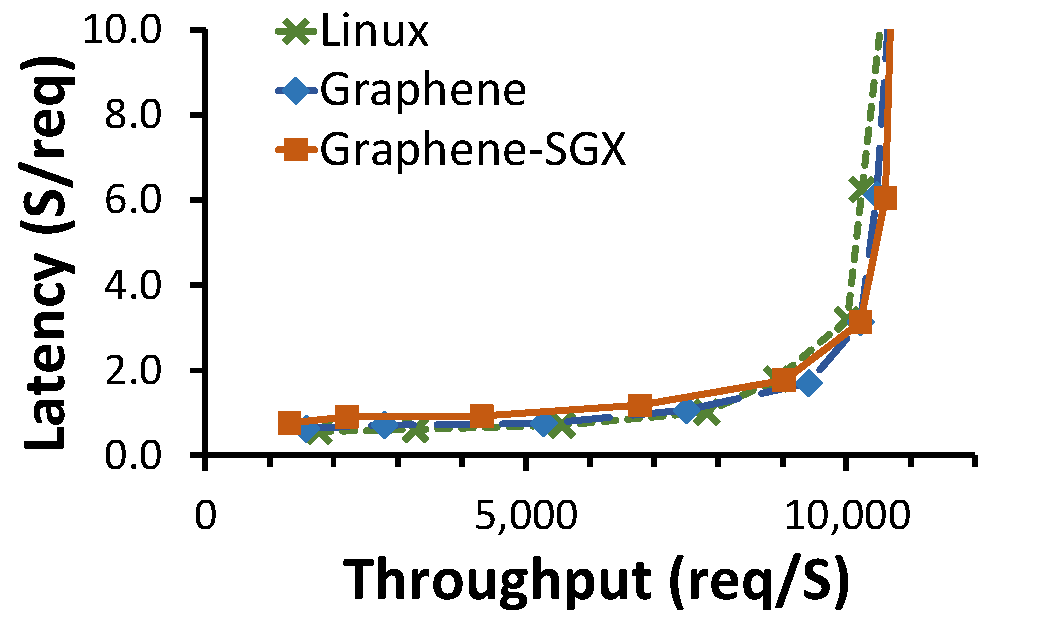
\includegraphics[width=\linewidth]{sgx/lighttpd-throughput-latency}\\
\vspace{3pt}
{\bf (a) Lighttpd (25 threads)}
\vspace{6pt}
\end{minipage}
\begin{minipage}{.45\textwidth}
\centering
\footnotesize
\vspace{6pt}
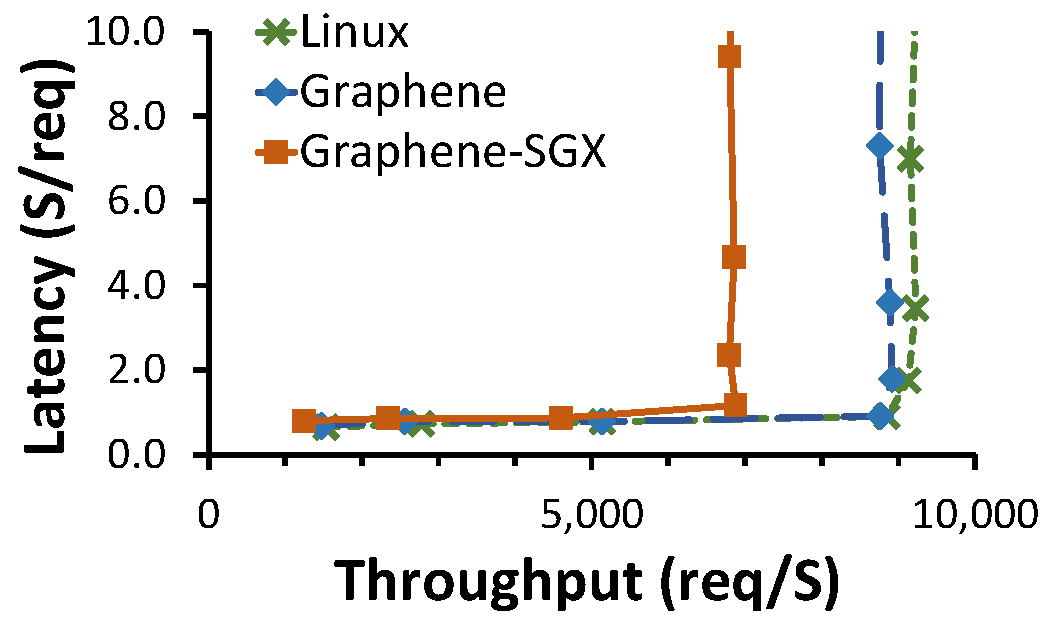
\includegraphics[width=\linewidth]{sgx/apache-throughput-latency}\\
\vspace{3pt}
{\bf (b) Apache (5 processes)}
\vspace{6pt}
\end{minipage}
\begin{minipage}{.45\textwidth}
\centering
\footnotesize
\vspace{6pt}
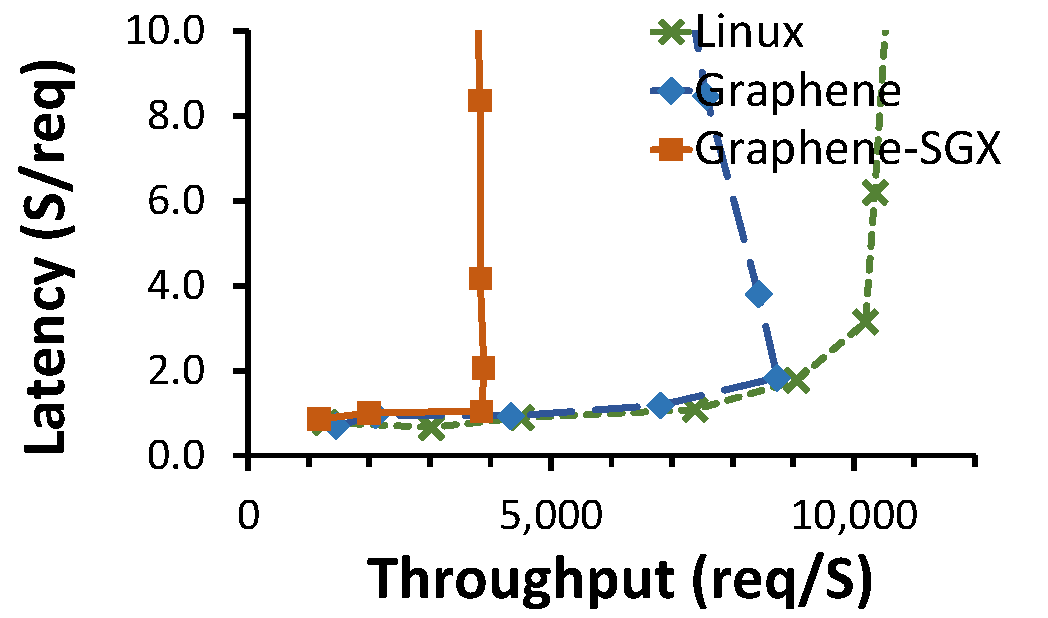
\includegraphics[width=\linewidth]{sgx/nginx-throughput-latency}\\
\vspace{3pt}
{\bf (c) NGINX (event-driven)}
\vspace{6pt}
\end{minipage}

\caption{Throughput versus latency of web server workloads, including Lighttpd, Apache, and NGINX, on native Linux, \graphene{}, and \graphenesgx{}.
We use an ApacheBench client to gradually increase load, and plot
throughput versus latency at each point.  Lower and further right
is better.
%\fixmedp{RB: Add another sentence or two to explain what the experiment is and how to interpret} }
}
\label{fig:server-throughput-latency}
\end{figure*}


{\bf Lighttpd}~\cite{lighttpd} is a web server designed to be light-weight, yet robust enough for commercial uses. 
Lighttpd is multi-threaded; we test with 25 threads to process HTTP requests. 
By default, Lighttpd uses the \syscall{epoll\_wait} system call to poll listening sockets.
At peak throughput and load,  both \graphene{} and \graphenesgx{} have marginal overhead on either latency or throughput of the Lighttpd server.
The overheads of \graphene{} are more apparent when the system
is more lightly loaded, at 
%When Lighttpd is not overloaded, \graphenesgx{} causes 
15--35\% higher response time, or 13--26\% lower throughput. 
Without SGX, \graphene{} induces 
11--15\% higher latency or 13-17\% lower throughput over Linux;
the remaining overheads are attributable to SGX---either hardware or our OS shield.
%platform adaptation layer (PAL) code.

%\fixmedp{Some more detailed analysis would be nice.}
%Only part of this overhead is contributed by the library OS implementation, since using \graphene{} without \sgx{} causes only 

%\fixmedp{Why did you comment this out?  Let's discuss: Does it really make sense to have two points at the same  x-axis value?  Perhaps the axes should be inverted?  I'm not really sure about the methodology, but something about the line doubling back on itself seems wrong.  Maybe you want to separate these and show throughput vs. load, and a CDF of latencies?}


{\bf Apache}~\cite{apache} is one of the most popular production web servers. We test Apache using 5 preforked worker processes to service HTTP requests,
in order to 
to evaluate the efficiency of \graphenesgx{} across enclaves.
%n server, 
%In the experiment, the Apache server creates 5 preforked processes which coordinate on processing HTTP requests.
This application uses IPC extensively---the preforked processes of a server use a System V semaphore to synchronize on each connection.
%When receiving a connection, the preforked processes of Apache will coordinate among themselves using the system V IPC semaphores.
Regardless of the workload, the response time on \graphenesgx{} is 12--35\% higher than Linux, due to the overhead of coordination across enclaves over encrypted RPC streams.
The peak throughput achieved by Apache running in \graphenesgx{} is 26\% lower than running in Linux.
In this workload, most of the overheads are SGX-specific, such as exiting enclaves when accessing the RPC, as non-SGX Graphene
has only 2--8\% overhead compared to Linux.

%The enclave restriction \fixmedp{Huh?} is the main contributor to this overhead, as \graphene{} generally only causes 2--8\% overhead.

%\fixmedp{Check the lightttp graph; the lines are right on top of each other, and dont' look 22\% apart to me.  Some of this may be the scale of the y axis}

{\bf NGINX}~\cite{nginx} is a relatively new web server designed for high programmability, for as a building block to implement different services.
Unlike the other two web servers, NGINX is event-driven and mostly configured as single-threaded.
%When running as a simple HTTP server, NGINX uses an event-driven model instead of multi-threading/multi-processing to handle incoming requests.
\graphenesgx{} currently only supports synchronous I/O at the enclave boundary,
and so, under load, it cannot as effectively overlap I/O and computation
as other systems that have batched and asynchronous system calls.
%Asynchronous system calls and events in general are less mature features of
%\graphenesgx{}, and, 
Once sufficiently loaded, NGINX on both \graphene{} and \graphenesgx{} 
performs worse than in a  Linux process. % once sufficiently loaded.
%We observe that both \graphene{} and \graphenesgx{} tend to perform poorly in an event-driven server.
The peak throughput of \graphenesgx{} is 1.5$\times$ lower than Linux;
without SGX, Graphene only reaches 79\% of Linux's peak throughput.
%\fixmedp{Maybe shout out to eleos, or cite other work}
We expect that using tools like Eleos~\cite{orenbach17eleos} to reduce exits
would help this workload; in future work, we will improve
asynchronous I/O in \graphenesgx{}.

%\graphenesgx{} causes 17--90\% more response time when the server is not overloaded,
%but up to 1.5$\times$ at the peak throughput.
%If we compare the peak throughput with native Linux, \graphenesgx{} is 70\% less.
%\graphene{} also suffers the same performance pattern, as the throughput drops dramatically after reaching 79\% of the peak throughput of NGINX in Linux.
%The reason of the slowdown is that the host interface of \graphene{} and \graphenesgx{} only supports synchronous IO, so implementing asynchronous IO will be less efficient. This limitation is a trade-off to the portability of \graphene{}.
%\fixmedp{Didn't get the portability point; please spell out what you meant, if important}


\begin{figure}[t!]
\centering
\footnotesize
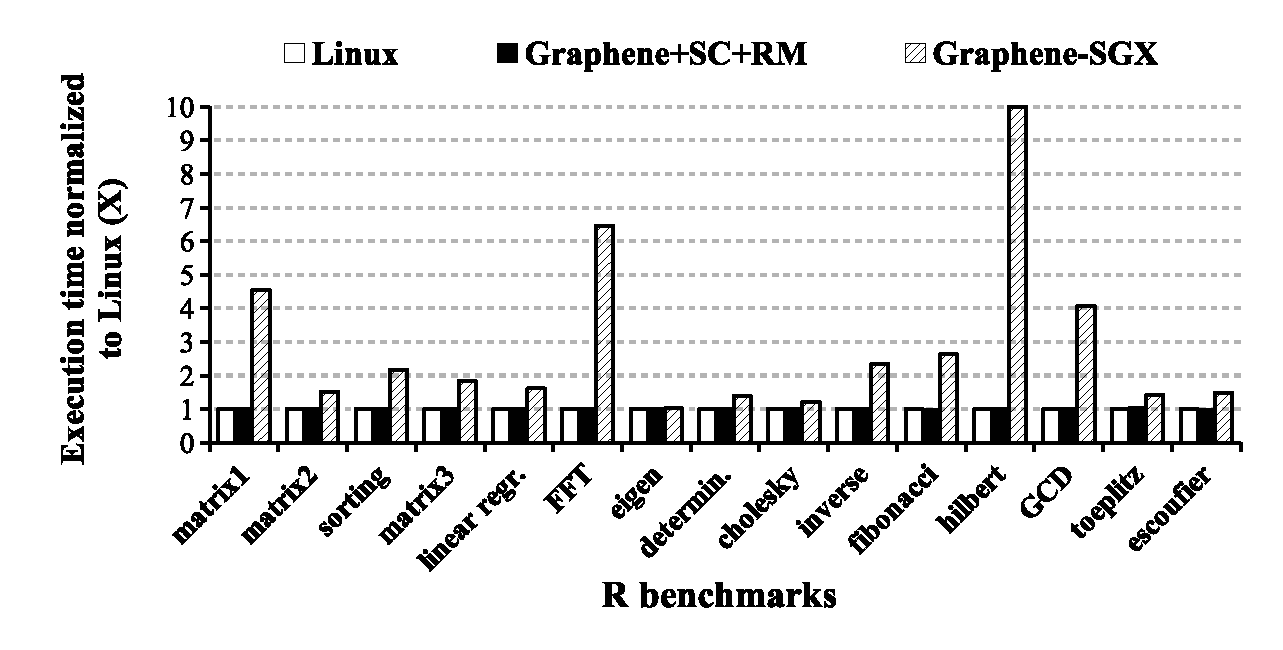
\includegraphics[width=38em]{r-overhead}\\
\caption{Performance overhead on desktop applications, including latency of R, execution time of GCC compilation, download time with CURL. The evaluation compares native Linux, \graphene{}, and \graphenesgx{}.} %{\bf Enclave creation time is deducted from the GCC execution time.}}
\label{fig:eval:r-overheads}
\end{figure}


\begin{figure}[t!]
\centering
\footnotesize
\begin{minipage}{.49\textwidth}
\centering
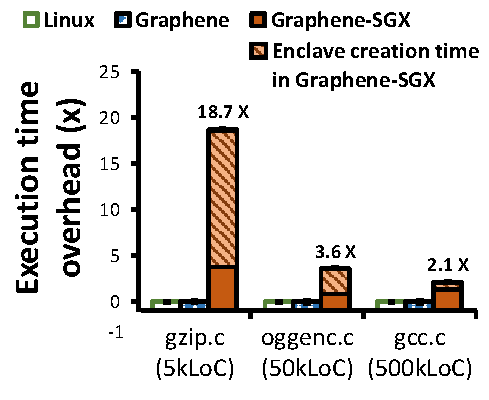
\includegraphics[width=20em]{sgx/gcc-overhead}\\
\vspace{3pt}
{\bf (b) GCC}
\end{minipage}
\begin{minipage}{.49\textwidth}
\centering
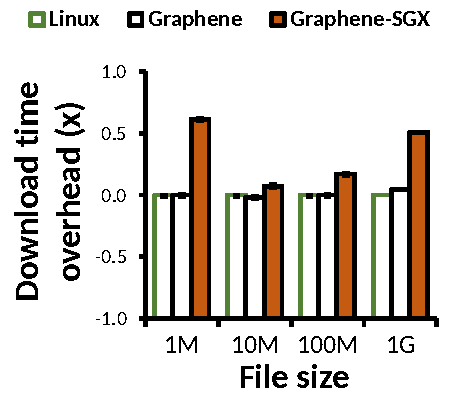
\includegraphics[width=20em]{sgx/curl-overhead}\\
\vspace{3pt}
{\bf (c) CURL}
\end{minipage}
\caption{Performance overhead on desktop applications, including latency of R, execution time of GCC compilation, download time with CURL. The evaluation compares native Linux, \graphene{}, and \graphenesgx{}.} %{\bf Enclave creation time is deducted from the GCC execution time.}}
\label{fig:desktop-overhead}
\end{figure}



\paragraph{Command-line applications}


We also evaluate the performance of a few commonly-used command-line applications.
%, to evaluate the performance of \graphenesgx{} on PCs instead of servers and clouds.
Three off-the-shelf applications are tested in our experiments:
{\bf R} (v3.2.3) for statistical computing~\cite{r-project}; {\bf GCC} (v5.4), the general GNU C compiler~\cite{gcc}; {\bf CURL} (v7.74), the default command-line web client on UNIX~\cite{curl}.
These applications are chosen because they are frequently used by Linux users,
and each of them potentially  be used 
in an enclave to handle sensitive data---either on a server or a client
machine.
% can realize profitable scenarios of using enclaves on desktop machines.



We evaluate the latency or execution time of these applications. 
%, because desktop users tend to care more about responsiveness than throughput.
In our experiments, both R and CURL have internal timing features to measure the wall time
of individual operations or executions.
%However, for other applications like GCC which does not include internal timing, evaluating the execution time can be influenced by many factors.
On a Linux host, the time to start a library OS is higher than a simple 
process, but significantly lower than booting a guest OS in a VM or
starting a container. 
Prior work measured Graphene (non-SGX) start time at 641 $\mu$s~\cite{tsai14graphene}, whereas starting an empty Linux VM takes 10.3s and starting a Linux (LXC) container takes 200 ms~\cite{agarwal15container}. 
%% dp; Note that this is MILLI seconds, not micro seconds.
%average memory footprint of an empty Linux VM, with memory deduplication, is about 96MB, . 


On SGX, the enclave creation time is relatively higher, \fixme{added more detailed number} ranging from 0.5s (a 256MB enclave) to 5s (a 2G enclave), which is a fixed cost that any application framework
will have to pay to run on SGX.
%For library OSes, the time for creating and initializing an enclave is not trivial, because it is similar to booting an lightweight OS.
% a significant part of the start-up time
% of an application is more significant, because creating enclaves is expensive.
%We consider the enclave creation time as a fixed cost for any application running in \graphenesgx{},
%and acceptable to users as long as it is responsive.
Enclave creation time is determined by the latency of the hardware and the Intel kernel driver, and is primarily a function of the size of 
the enclave, which is specified at creation time because it affects the enclave signature. %\fixmedp{although can't it grow with eadd?}.  
For non-server workloads that create multiple processes during execution,
such as GCC in Figure~\ref{fig:desktop-overhead},
the enclave creation contributes a significant portion to the execution time overheads, illustrated as a stacked bar.
%Since the enclave creation time is related to the enclave size, and unrelated to the workload,
%we deduct the enclave creation time from the execution time of GCC in Figure~\ref{fig:desktop-overhead}. \fixmedp{I think it might be better to show this as a stacked bar instead of just removing it.  Opaquely subtracting this cost doesn't seem right.  Let's discuss dp: I thought we agreed to change this...}

{\bf R}~\cite{r-project} is a scripting language often used for
data processing and statistical computation.
With enclaves, users can process sensitive data on an
OS they don't trust.
We use an R benchmark suite developed by Urbanek et al.~\cite{r-benchmark-25}, which includes 15 CPU-bound workloads such as matrix computation and number processing.
\graphenesgx{} slows down by less than 100\% on the majority of the workloads, excepts the ones which involve allocation and garbage collection: ({\tt matrix1} creates and destroys matrices, and both {\tt FFT} and {\tt hilbert} involve heavy garbage collection.)
Aside from garbage collection, these R benchmarks do not frequently interact with the host.
We further note that non-SGX \graphene{} is as efficient as Linux on all workloads, 
and these overheads appear to be SGX-specific.
%\fixmedp{Check this pontification}
In our experience, garbage collection and memory management code in managed language runtime
systems tends to be written with assumptions that do not match enclaves,
such as a large, sparse address space or that memory can be demand paged 
nearly for free (SGX version 1 requires all memory to be mapped
at creation); a useful area for future work would be to design
garbage collection strategies that are optimized for enclaves.
%we believe the overheads on \graphenesgx{} are contributed by enclaves.

{\bf GCC}~\cite{gcc} is a widely-used C compiler.
By supporting GCC in enclaves, developers can compile closed-source applications on customers' machines,
without leaking the source code.
GCC composes of multiple binaries, including {\tt cc1} (compiler), {\tt as} (assembler), and {\tt ld} (linker).
Therefore, GCC is a multi-process program using \syscall{execve}.
We test the compilation of thee source files with varied sizes,
using single C source files collected by MIT~\cite{gcc-benchmark}.
Each GCC execution typically \fixme{it's five, not four} creates five processes, and we run each process in a 256MB enclave by default.
%and has a fixed cost on enclave creation, which is unrelated to workload and depends on the enclave size.
%\fixme{check this}
\fixme{clarified this part, to prevent confusion between latency and overhead. also, GCC numbers got better.}
For a small workload like compiling {\tt gzip.c} (5 kLoC), running in \graphenesgx{} (4.1s) is 18.7$\times$ slower than Linux (0.2s).
The bulk of this time is spent in enclave creation, taking 3.0s in total, while the whole execution inside the enclaves, including initialization of the library OS and OS shield, takes only 1.1s, or 4.2$\times$ overhead.
For larger workloads like {\tt oggenc.c} (50 kLoC) and {\tt gcc.c} (500 kLoC), 
the overhead of \graphenesgx{} is less significant. % (3.6$\times$ and 2.1$\times$ overhead, respectively).
For {\tt gcc.c} (500 kLoC), we have to enlarge one of the enclaves ({\tt cc1}) to 2GB,
but running on \graphenesgx{} (53.1s) is only 2.1$\times$ slower than Linux (17.2s),
and 7.1s is spent on enclave creation.
%and the creation of four enclaves takes 8s.
%Each compilation has a fixed enclave creation time in \graphenesgx{}, which is about 1--2 seconds per enclave. We deduct the creation time of all enclaves  to gain more meaningful results, but do not hide rest of the overhead on fork.
%\fixmedp{Also not comfortable with this; add a bar?}
%In general, GCC in \graphenesgx{} is 1--5$\times$ slower than GCC on native Linux. 
%\fixmedp{This really needs some profiling if possible}
The overhead of non-SGX \graphene{} on GCC is marginal.




{\bf CURL}~\cite{curl} is a command-line  web downloader.
\graphenesgx{} can make CURL into a secure downloader that attests both server and client ends.
We evaluate the total time to download a large file, ranging from 1MB to 1GB, from another machine running Apache. % over Gigabit LAN.
%across high-speed university network\fixmedp{more specific, as above}.
\graphene{} has marginal overhead on CURL, and
\graphenesgx{} adds 7--61\% overhead to the downloading time of CURL, due to the latency of I/O.


\caption{Application benchmark execution times in a (1) native Linux process, (2) a process inside a KVM virtual machine, (3) a \graphene{} \picoproc{} with the SECCOMP filter ({\bf +SC}) and reference monitor ({\bf +RM}). }
\label{tab:graphene:apps}
\end{table}



Table~\ref{tab:graphene:apps} lists 
execution time of our {\em unmodified} 
application benchmarks (detailed in \S\ref{sec:eval:graphene}).
All applications create multiple processes,
except for \lighttpd{}, which only creates multiple threads.
Each data point is the average of at least six runs, 
and 95\% confidence intervals are listed in the table.

We exercise  {\tt \gcc{}}/{\tt make}
with inputs of varying sizes:
%the pbzip2 compression utility (v1.1.6, 4 KLoC),
%the ogg sound encoder (v1.0.1, 5 KLoC),
%GNU {\tt make} (v3.82, \fixmedp{XX} KLoC)
bzip2 (v1.0.6, 5KLoC, 13 files),
\graphene{}'s {\tt libLinux} (31 KLoC, 78 files)
and \gcc{} (v3.5.0, 551 KLoC, collected as a single source file). 
We benchmark Apache (4 preforked workers) and \lighttpd{} (4 threads) with 
\ab{},
which issues 25, 50, and 100 concurrent requests
to download a 100 byte file 50,000 times.

We exercised \busy{} with 
300 iterations of the Unixbench benchmark~\cite{unixbench}, as well as 
300 iterations of a simple shell script benchmark that runs 6 common shell script commands
({\tt cp}, {\tt rm}, {\tt ls}, {\tt cat}, {\tt date}, and {\tt echo}).

Compilation workloads incur overheads ranging from 5--30\%.
%All compilation workloads have minimal overheads compared to native when executed sequentially;
Parallel compilation on both \graphene{} and Linux yields comparable  speedups  over sequential,
but the percent overhead increases for parallel \graphene{}.
For instance, {\tt make -j4 libLinux} speeds up 3.7\x{} on Linux and 3.4$\times$ on \graphene{}.
The compilation overheads are primarily from the reference monitor---nearly all for bzip2 and gcc, and half for {\tt libLinux}.
%Nearly all of the overhead from the bzip2 and gcc compilations are from the reference monitor; about half of the overheads of {\tt libLinux} compile 
%are the reference monitor and half are \graphene{} itself.
In the case of both \busy{} workloads, the key bottleneck is the {\tt fork} system call.
Profiling indicates that half of the time in {\tt libLinux} is spent on {\tt fork} in both benchmarks.
The trend is exacerbated in Unixbench, which creates all of the processes at the beginning and
waits for them all to complete; because \graphene{} cannot create children as quickly as native, this leads to 
load imbalance throughout the rest of the benchmark.  

With the reference monitor disabled,  \lighttpd{} has equivalent throughput to a native Linux process;
as discussed in the next subsection, these overheads come from checking paths in the monitor.
The Apache web server loses about half of its throughput relative to \lighttpd{} on \graphene{}.
The primary bottleneck in Apache relative to \lighttpd{} is System V semaphores,
%, which account for about 
%one third of the additional time spent in {\tt libLinux}
%relative to \light{}, 
and the remaining overheads are attributable to more time spent waiting for input.
The overheads for both \lighttpd{} and Apache on KVM are primarily attributable
to bridged networking.


One deployment model for SGX is to host network services
on an untrusted cloud provider's hardware.
%To measure this case, 
We measure three widely-used Linux web servers, including {\bf Lighttpd}~\cite{lighttpd} (v1.4.35), {\bf Apache}~\cite{apache} (v2.4.18), and {\bf NGINX}~\cite{nginx} (v1.10).
%, to evaluate the performance of server-type workloads in \graphenesgx{}.
%These applications are all sophisticated, non-trivial workloads, and are constantly being used for commercial purposes.
%We test these applications to evaluating significantly different execution patterns, to benchmark the performance of \graphenesgx{} under each circumstances.
%Also, we do not explicitly configure these servers to secure their payloads using the HTTPS protocol.\fixme{if have time, maybe try again with HTTPS}
For each workload, we use ApacheBench~\cite{apachebench} to download the web pages on a separate machine.
%\edit{over Gigabit LAN}. %\fixmedp{more specific?}
%across a high-speed \fixmedp{Can you say
%more specifically the specs, like 10 GBps or whatever; also, if this is the same vlan, I might just describe this as being on a LAN, minimizing interference} University network.
The concurrency of ApacheBench is gradually increased during the experiment, to test the both the per-request latency and the overall throughput of the server.
Figure~\ref{fig:server-throughput-latency} shows the throughput versus latency of these server applications
in \graphenesgx{}, \graphene{} and Linux. 
Each workload is discussed below.




% Put figures at the front
\begin{figure*}[t!]
\centering

\begin{minipage}{.45\textwidth}
\centering
\footnotesize
\vspace{6pt}
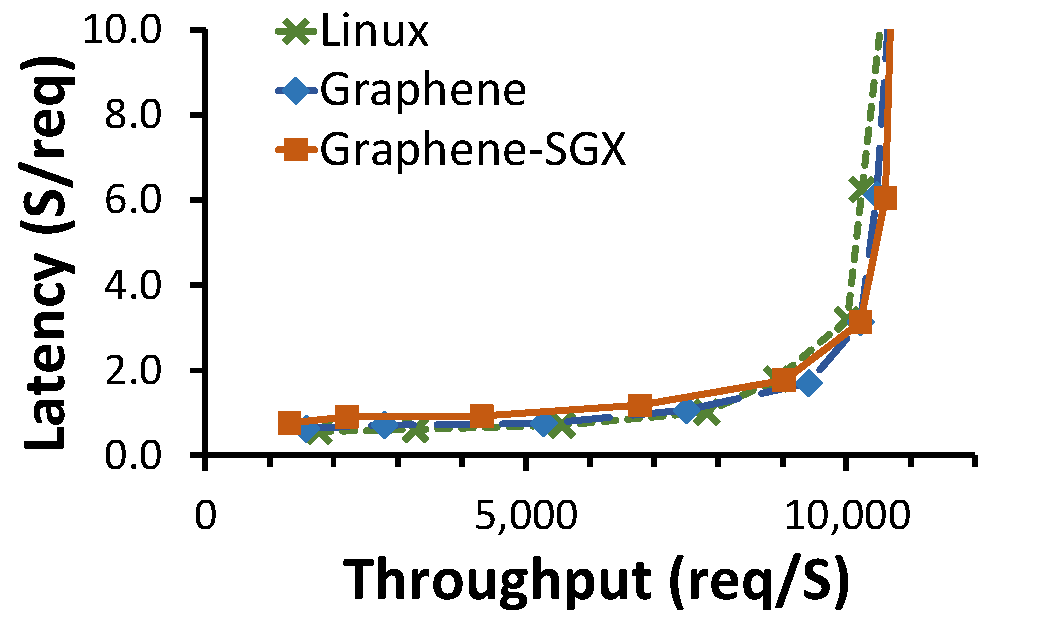
\includegraphics[width=\linewidth]{sgx/lighttpd-throughput-latency}\\
\vspace{3pt}
{\bf (a) Lighttpd (25 threads)}
\vspace{6pt}
\end{minipage}
\begin{minipage}{.45\textwidth}
\centering
\footnotesize
\vspace{6pt}
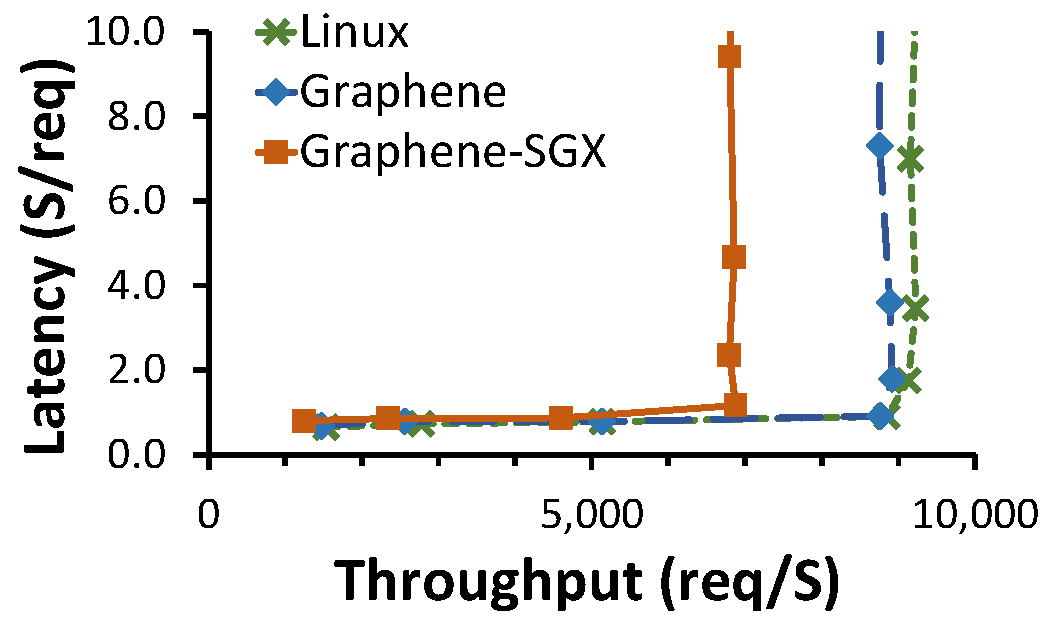
\includegraphics[width=\linewidth]{sgx/apache-throughput-latency}\\
\vspace{3pt}
{\bf (b) Apache (5 processes)}
\vspace{6pt}
\end{minipage}
\begin{minipage}{.45\textwidth}
\centering
\footnotesize
\vspace{6pt}
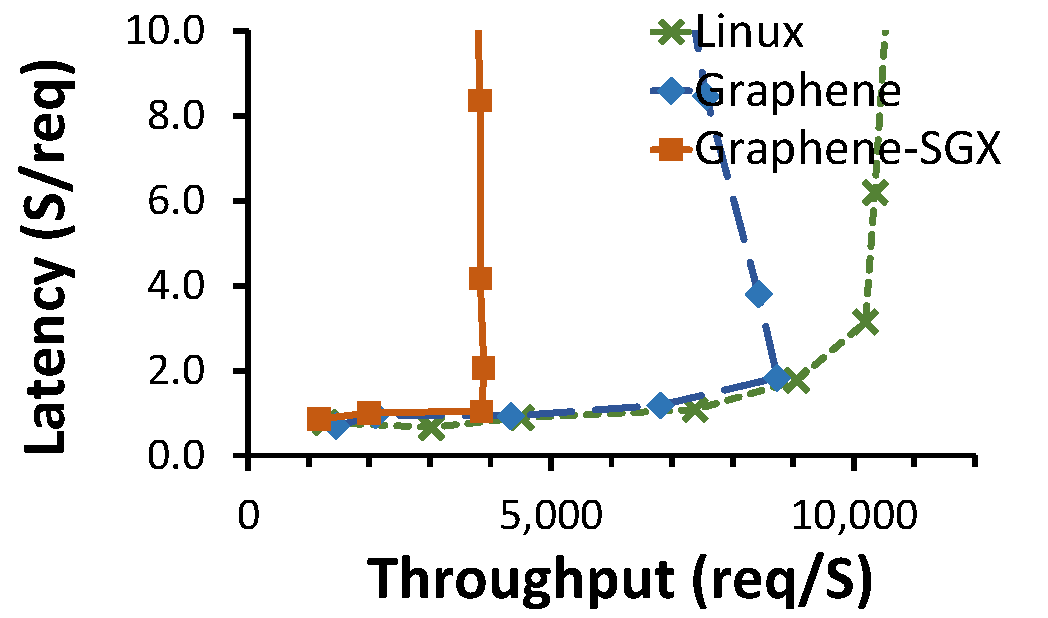
\includegraphics[width=\linewidth]{sgx/nginx-throughput-latency}\\
\vspace{3pt}
{\bf (c) NGINX (event-driven)}
\vspace{6pt}
\end{minipage}

\caption{Throughput versus latency of web server workloads, including Lighttpd, Apache, and NGINX, on native Linux, \graphene{}, and \graphenesgx{}.
We use an ApacheBench client to gradually increase load, and plot
throughput versus latency at each point.  Lower and further right
is better.
%\fixmedp{RB: Add another sentence or two to explain what the experiment is and how to interpret} }
}
\label{fig:server-throughput-latency}
\end{figure*}


{\bf Lighttpd}~\cite{lighttpd} is a web server designed to be light-weight, yet robust enough for commercial uses. 
Lighttpd is multi-threaded; we test with 25 threads to process HTTP requests. 
By default, Lighttpd uses the \syscall{epoll\_wait} system call to poll listening sockets.
At peak throughput and load,  both \graphene{} and \graphenesgx{} have marginal overhead on either latency or throughput of the Lighttpd server.
The overheads of \graphene{} are more apparent when the system
is more lightly loaded, at 
%When Lighttpd is not overloaded, \graphenesgx{} causes 
15--35\% higher response time, or 13--26\% lower throughput. 
Without SGX, \graphene{} induces 
11--15\% higher latency or 13-17\% lower throughput over Linux;
the remaining overheads are attributable to SGX---either hardware or our OS shield.
%platform adaptation layer (PAL) code.

%\fixmedp{Some more detailed analysis would be nice.}
%Only part of this overhead is contributed by the library OS implementation, since using \graphene{} without \sgx{} causes only 

%\fixmedp{Why did you comment this out?  Let's discuss: Does it really make sense to have two points at the same  x-axis value?  Perhaps the axes should be inverted?  I'm not really sure about the methodology, but something about the line doubling back on itself seems wrong.  Maybe you want to separate these and show throughput vs. load, and a CDF of latencies?}


{\bf Apache}~\cite{apache} is one of the most popular production web servers. We test Apache using 5 preforked worker processes to service HTTP requests,
in order to 
to evaluate the efficiency of \graphenesgx{} across enclaves.
%n server, 
%In the experiment, the Apache server creates 5 preforked processes which coordinate on processing HTTP requests.
This application uses IPC extensively---the preforked processes of a server use a System V semaphore to synchronize on each connection.
%When receiving a connection, the preforked processes of Apache will coordinate among themselves using the system V IPC semaphores.
Regardless of the workload, the response time on \graphenesgx{} is 12--35\% higher than Linux, due to the overhead of coordination across enclaves over encrypted RPC streams.
The peak throughput achieved by Apache running in \graphenesgx{} is 26\% lower than running in Linux.
In this workload, most of the overheads are SGX-specific, such as exiting enclaves when accessing the RPC, as non-SGX Graphene
has only 2--8\% overhead compared to Linux.

%The enclave restriction \fixmedp{Huh?} is the main contributor to this overhead, as \graphene{} generally only causes 2--8\% overhead.

%\fixmedp{Check the lightttp graph; the lines are right on top of each other, and dont' look 22\% apart to me.  Some of this may be the scale of the y axis}

{\bf NGINX}~\cite{nginx} is a relatively new web server designed for high programmability, for as a building block to implement different services.
Unlike the other two web servers, NGINX is event-driven and mostly configured as single-threaded.
%When running as a simple HTTP server, NGINX uses an event-driven model instead of multi-threading/multi-processing to handle incoming requests.
\graphenesgx{} currently only supports synchronous I/O at the enclave boundary,
and so, under load, it cannot as effectively overlap I/O and computation
as other systems that have batched and asynchronous system calls.
%Asynchronous system calls and events in general are less mature features of
%\graphenesgx{}, and, 
Once sufficiently loaded, NGINX on both \graphene{} and \graphenesgx{} 
performs worse than in a  Linux process. % once sufficiently loaded.
%We observe that both \graphene{} and \graphenesgx{} tend to perform poorly in an event-driven server.
The peak throughput of \graphenesgx{} is 1.5$\times$ lower than Linux;
without SGX, Graphene only reaches 79\% of Linux's peak throughput.
%\fixmedp{Maybe shout out to eleos, or cite other work}
We expect that using tools like Eleos~\cite{orenbach17eleos} to reduce exits
would help this workload; in future work, we will improve
asynchronous I/O in \graphenesgx{}.

%\graphenesgx{} causes 17--90\% more response time when the server is not overloaded,
%but up to 1.5$\times$ at the peak throughput.
%If we compare the peak throughput with native Linux, \graphenesgx{} is 70\% less.
%\graphene{} also suffers the same performance pattern, as the throughput drops dramatically after reaching 79\% of the peak throughput of NGINX in Linux.
%The reason of the slowdown is that the host interface of \graphene{} and \graphenesgx{} only supports synchronous IO, so implementing asynchronous IO will be less efficient. This limitation is a trade-off to the portability of \graphene{}.
%\fixmedp{Didn't get the portability point; please spell out what you meant, if important}


\begin{figure}[t!]
\centering
\footnotesize
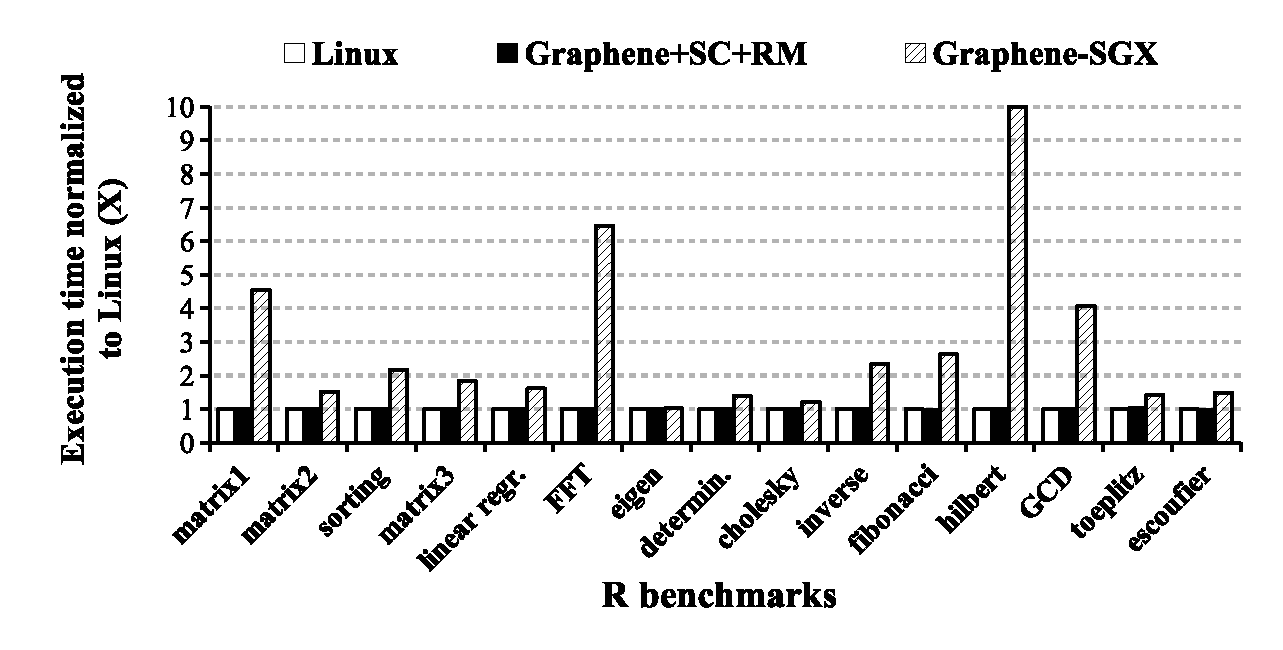
\includegraphics[width=38em]{r-overhead}\\
\caption{Performance overhead on desktop applications, including latency of R, execution time of GCC compilation, download time with CURL. The evaluation compares native Linux, \graphene{}, and \graphenesgx{}.} %{\bf Enclave creation time is deducted from the GCC execution time.}}
\label{fig:eval:r-overheads}
\end{figure}


\begin{figure}[t!]
\centering
\footnotesize
\begin{minipage}{.49\textwidth}
\centering
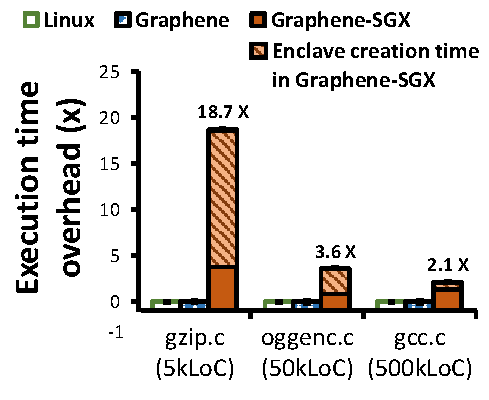
\includegraphics[width=20em]{sgx/gcc-overhead}\\
\vspace{3pt}
{\bf (b) GCC}
\end{minipage}
\begin{minipage}{.49\textwidth}
\centering
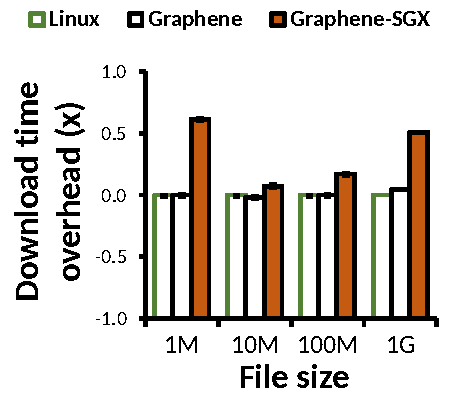
\includegraphics[width=20em]{sgx/curl-overhead}\\
\vspace{3pt}
{\bf (c) CURL}
\end{minipage}
\caption{Performance overhead on desktop applications, including latency of R, execution time of GCC compilation, download time with CURL. The evaluation compares native Linux, \graphene{}, and \graphenesgx{}.} %{\bf Enclave creation time is deducted from the GCC execution time.}}
\label{fig:desktop-overhead}
\end{figure}



\paragraph{Command-line applications}


We also evaluate the performance of a few commonly-used command-line applications.
%, to evaluate the performance of \graphenesgx{} on PCs instead of servers and clouds.
Three off-the-shelf applications are tested in our experiments:
{\bf R} (v3.2.3) for statistical computing~\cite{r-project}; {\bf GCC} (v5.4), the general GNU C compiler~\cite{gcc}; {\bf CURL} (v7.74), the default command-line web client on UNIX~\cite{curl}.
These applications are chosen because they are frequently used by Linux users,
and each of them potentially  be used 
in an enclave to handle sensitive data---either on a server or a client
machine.
% can realize profitable scenarios of using enclaves on desktop machines.



We evaluate the latency or execution time of these applications. 
%, because desktop users tend to care more about responsiveness than throughput.
In our experiments, both R and CURL have internal timing features to measure the wall time
of individual operations or executions.
%However, for other applications like GCC which does not include internal timing, evaluating the execution time can be influenced by many factors.
On a Linux host, the time to start a library OS is higher than a simple 
process, but significantly lower than booting a guest OS in a VM or
starting a container. 
Prior work measured Graphene (non-SGX) start time at 641 $\mu$s~\cite{tsai14graphene}, whereas starting an empty Linux VM takes 10.3s and starting a Linux (LXC) container takes 200 ms~\cite{agarwal15container}. 
%% dp; Note that this is MILLI seconds, not micro seconds.
%average memory footprint of an empty Linux VM, with memory deduplication, is about 96MB, . 


On SGX, the enclave creation time is relatively higher, \fixme{added more detailed number} ranging from 0.5s (a 256MB enclave) to 5s (a 2G enclave), which is a fixed cost that any application framework
will have to pay to run on SGX.
%For library OSes, the time for creating and initializing an enclave is not trivial, because it is similar to booting an lightweight OS.
% a significant part of the start-up time
% of an application is more significant, because creating enclaves is expensive.
%We consider the enclave creation time as a fixed cost for any application running in \graphenesgx{},
%and acceptable to users as long as it is responsive.
Enclave creation time is determined by the latency of the hardware and the Intel kernel driver, and is primarily a function of the size of 
the enclave, which is specified at creation time because it affects the enclave signature. %\fixmedp{although can't it grow with eadd?}.  
For non-server workloads that create multiple processes during execution,
such as GCC in Figure~\ref{fig:desktop-overhead},
the enclave creation contributes a significant portion to the execution time overheads, illustrated as a stacked bar.
%Since the enclave creation time is related to the enclave size, and unrelated to the workload,
%we deduct the enclave creation time from the execution time of GCC in Figure~\ref{fig:desktop-overhead}. \fixmedp{I think it might be better to show this as a stacked bar instead of just removing it.  Opaquely subtracting this cost doesn't seem right.  Let's discuss dp: I thought we agreed to change this...}

{\bf R}~\cite{r-project} is a scripting language often used for
data processing and statistical computation.
With enclaves, users can process sensitive data on an
OS they don't trust.
We use an R benchmark suite developed by Urbanek et al.~\cite{r-benchmark-25}, which includes 15 CPU-bound workloads such as matrix computation and number processing.
\graphenesgx{} slows down by less than 100\% on the majority of the workloads, excepts the ones which involve allocation and garbage collection: ({\tt matrix1} creates and destroys matrices, and both {\tt FFT} and {\tt hilbert} involve heavy garbage collection.)
Aside from garbage collection, these R benchmarks do not frequently interact with the host.
We further note that non-SGX \graphene{} is as efficient as Linux on all workloads, 
and these overheads appear to be SGX-specific.
%\fixmedp{Check this pontification}
In our experience, garbage collection and memory management code in managed language runtime
systems tends to be written with assumptions that do not match enclaves,
such as a large, sparse address space or that memory can be demand paged 
nearly for free (SGX version 1 requires all memory to be mapped
at creation); a useful area for future work would be to design
garbage collection strategies that are optimized for enclaves.
%we believe the overheads on \graphenesgx{} are contributed by enclaves.

{\bf GCC}~\cite{gcc} is a widely-used C compiler.
By supporting GCC in enclaves, developers can compile closed-source applications on customers' machines,
without leaking the source code.
GCC composes of multiple binaries, including {\tt cc1} (compiler), {\tt as} (assembler), and {\tt ld} (linker).
Therefore, GCC is a multi-process program using \syscall{execve}.
We test the compilation of thee source files with varied sizes,
using single C source files collected by MIT~\cite{gcc-benchmark}.
Each GCC execution typically \fixme{it's five, not four} creates five processes, and we run each process in a 256MB enclave by default.
%and has a fixed cost on enclave creation, which is unrelated to workload and depends on the enclave size.
%\fixme{check this}
\fixme{clarified this part, to prevent confusion between latency and overhead. also, GCC numbers got better.}
For a small workload like compiling {\tt gzip.c} (5 kLoC), running in \graphenesgx{} (4.1s) is 18.7$\times$ slower than Linux (0.2s).
The bulk of this time is spent in enclave creation, taking 3.0s in total, while the whole execution inside the enclaves, including initialization of the library OS and OS shield, takes only 1.1s, or 4.2$\times$ overhead.
For larger workloads like {\tt oggenc.c} (50 kLoC) and {\tt gcc.c} (500 kLoC), 
the overhead of \graphenesgx{} is less significant. % (3.6$\times$ and 2.1$\times$ overhead, respectively).
For {\tt gcc.c} (500 kLoC), we have to enlarge one of the enclaves ({\tt cc1}) to 2GB,
but running on \graphenesgx{} (53.1s) is only 2.1$\times$ slower than Linux (17.2s),
and 7.1s is spent on enclave creation.
%and the creation of four enclaves takes 8s.
%Each compilation has a fixed enclave creation time in \graphenesgx{}, which is about 1--2 seconds per enclave. We deduct the creation time of all enclaves  to gain more meaningful results, but do not hide rest of the overhead on fork.
%\fixmedp{Also not comfortable with this; add a bar?}
%In general, GCC in \graphenesgx{} is 1--5$\times$ slower than GCC on native Linux. 
%\fixmedp{This really needs some profiling if possible}
The overhead of non-SGX \graphene{} on GCC is marginal.




{\bf CURL}~\cite{curl} is a command-line  web downloader.
\graphenesgx{} can make CURL into a secure downloader that attests both server and client ends.
We evaluate the total time to download a large file, ranging from 1MB to 1GB, from another machine running Apache. % over Gigabit LAN.
%across high-speed university network\fixmedp{more specific, as above}.
\graphene{} has marginal overhead on CURL, and
\graphenesgx{} adds 7--61\% overhead to the downloading time of CURL, due to the latency of I/O.


\caption{Application benchmark execution times in a (1) native Linux process, (2) a process inside a KVM virtual machine, (3) a \graphene{} \picoproc{} with the SECCOMP filter ({\bf +SC}) and reference monitor ({\bf +RM}). }
\label{tab:graphene:apps}
\end{table}



Table~\ref{tab:graphene:apps} lists 
execution time of our {\em unmodified} 
application benchmarks (detailed in \S\ref{sec:eval:graphene}).
All applications create multiple processes,
except for \lighttpd{}, which only creates multiple threads.
Each data point is the average of at least six runs, 
and 95\% confidence intervals are listed in the table.

We exercise  {\tt \gcc{}}/{\tt make}
with inputs of varying sizes:
%the pbzip2 compression utility (v1.1.6, 4 KLoC),
%the ogg sound encoder (v1.0.1, 5 KLoC),
%GNU {\tt make} (v3.82, \fixmedp{XX} KLoC)
bzip2 (v1.0.6, 5KLoC, 13 files),
\graphene{}'s {\tt libLinux} (31 KLoC, 78 files)
and \gcc{} (v3.5.0, 551 KLoC, collected as a single source file). 
We benchmark Apache (4 preforked workers) and \lighttpd{} (4 threads) with 
\ab{},
which issues 25, 50, and 100 concurrent requests
to download a 100 byte file 50,000 times.

We exercised \busy{} with 
300 iterations of the Unixbench benchmark~\cite{unixbench}, as well as 
300 iterations of a simple shell script benchmark that runs 6 common shell script commands
({\tt cp}, {\tt rm}, {\tt ls}, {\tt cat}, {\tt date}, and {\tt echo}).

Compilation workloads incur overheads ranging from 5--30\%.
%All compilation workloads have minimal overheads compared to native when executed sequentially;
Parallel compilation on both \graphene{} and Linux yields comparable  speedups  over sequential,
but the percent overhead increases for parallel \graphene{}.
For instance, {\tt make -j4 libLinux} speeds up 3.7\x{} on Linux and 3.4$\times$ on \graphene{}.
The compilation overheads are primarily from the reference monitor---nearly all for bzip2 and gcc, and half for {\tt libLinux}.
%Nearly all of the overhead from the bzip2 and gcc compilations are from the reference monitor; about half of the overheads of {\tt libLinux} compile 
%are the reference monitor and half are \graphene{} itself.
In the case of both \busy{} workloads, the key bottleneck is the {\tt fork} system call.
Profiling indicates that half of the time in {\tt libLinux} is spent on {\tt fork} in both benchmarks.
The trend is exacerbated in Unixbench, which creates all of the processes at the beginning and
waits for them all to complete; because \graphene{} cannot create children as quickly as native, this leads to 
load imbalance throughout the rest of the benchmark.  

With the reference monitor disabled,  \lighttpd{} has equivalent throughput to a native Linux process;
as discussed in the next subsection, these overheads come from checking paths in the monitor.
The Apache web server loses about half of its throughput relative to \lighttpd{} on \graphene{}.
The primary bottleneck in Apache relative to \lighttpd{} is System V semaphores,
%, which account for about 
%one third of the additional time spent in {\tt libLinux}
%relative to \light{}, 
and the remaining overheads are attributable to more time spent waiting for input.
The overheads for both \lighttpd{} and Apache on KVM are primarily attributable
to bridged networking.


One deployment model for SGX is to host network services
on an untrusted cloud provider's hardware.
%To measure this case, 
We measure three widely-used Linux web servers, including {\bf Lighttpd}~\cite{lighttpd} (v1.4.35), {\bf Apache}~\cite{apache} (v2.4.18), and {\bf NGINX}~\cite{nginx} (v1.10).
%, to evaluate the performance of server-type workloads in \graphenesgx{}.
%These applications are all sophisticated, non-trivial workloads, and are constantly being used for commercial purposes.
%We test these applications to evaluating significantly different execution patterns, to benchmark the performance of \graphenesgx{} under each circumstances.
%Also, we do not explicitly configure these servers to secure their payloads using the HTTPS protocol.\fixme{if have time, maybe try again with HTTPS}
For each workload, we use ApacheBench~\cite{apachebench} to download the web pages on a separate machine.
%\edit{over Gigabit LAN}. %\fixmedp{more specific?}
%across a high-speed \fixmedp{Can you say
%more specifically the specs, like 10 GBps or whatever; also, if this is the same vlan, I might just describe this as being on a LAN, minimizing interference} University network.
The concurrency of ApacheBench is gradually increased during the experiment, to test the both the per-request latency and the overall throughput of the server.
Figure~\ref{fig:server-throughput-latency} shows the throughput versus latency of these server applications
in \graphenesgx{}, \graphene{} and Linux. 
Each workload is discussed below.




% Put figures at the front
\begin{figure*}[t!]
\centering

\begin{minipage}{.45\textwidth}
\centering
\footnotesize
\vspace{6pt}
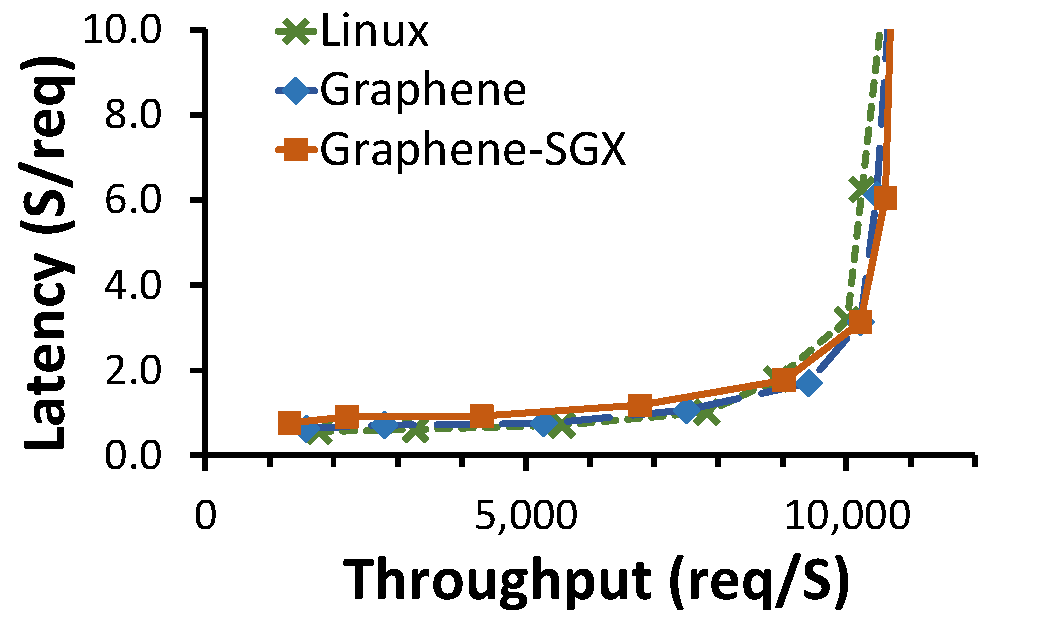
\includegraphics[width=\linewidth]{sgx/lighttpd-throughput-latency}\\
\vspace{3pt}
{\bf (a) Lighttpd (25 threads)}
\vspace{6pt}
\end{minipage}
\begin{minipage}{.45\textwidth}
\centering
\footnotesize
\vspace{6pt}
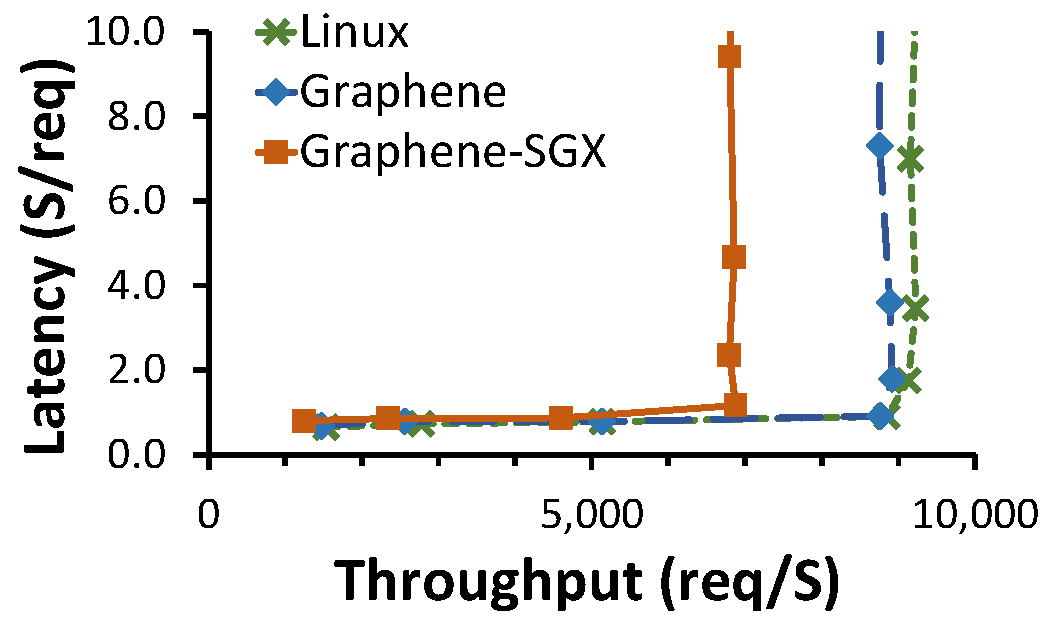
\includegraphics[width=\linewidth]{sgx/apache-throughput-latency}\\
\vspace{3pt}
{\bf (b) Apache (5 processes)}
\vspace{6pt}
\end{minipage}
\begin{minipage}{.45\textwidth}
\centering
\footnotesize
\vspace{6pt}
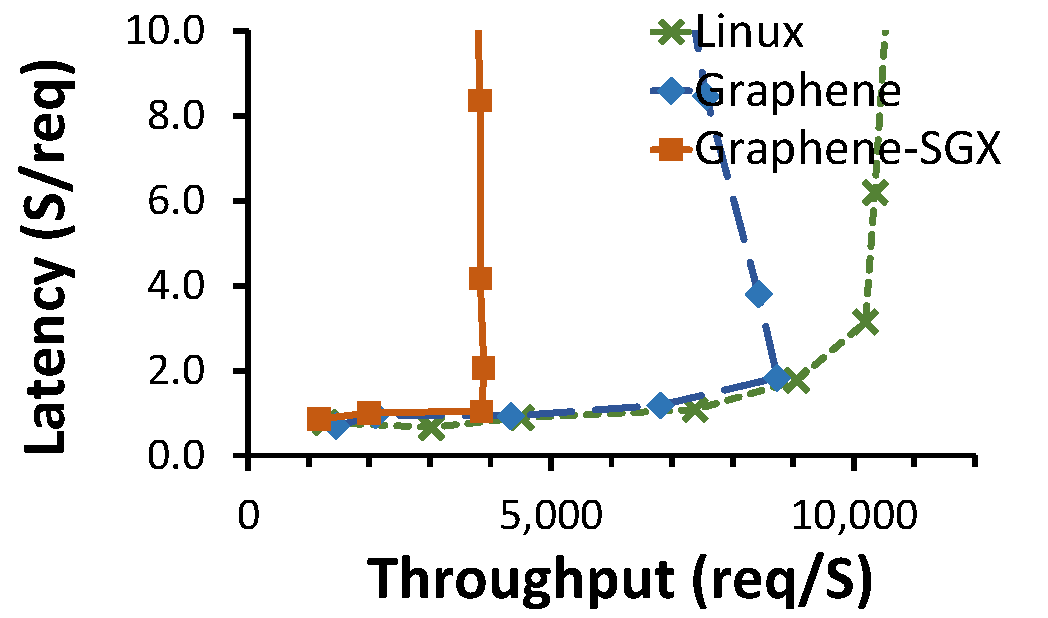
\includegraphics[width=\linewidth]{sgx/nginx-throughput-latency}\\
\vspace{3pt}
{\bf (c) NGINX (event-driven)}
\vspace{6pt}
\end{minipage}

\caption{Throughput versus latency of web server workloads, including Lighttpd, Apache, and NGINX, on native Linux, \graphene{}, and \graphenesgx{}.
We use an ApacheBench client to gradually increase load, and plot
throughput versus latency at each point.  Lower and further right
is better.
%\fixmedp{RB: Add another sentence or two to explain what the experiment is and how to interpret} }
}
\label{fig:server-throughput-latency}
\end{figure*}


{\bf Lighttpd}~\cite{lighttpd} is a web server designed to be light-weight, yet robust enough for commercial uses. 
Lighttpd is multi-threaded; we test with 25 threads to process HTTP requests. 
By default, Lighttpd uses the \syscall{epoll\_wait} system call to poll listening sockets.
At peak throughput and load,  both \graphene{} and \graphenesgx{} have marginal overhead on either latency or throughput of the Lighttpd server.
The overheads of \graphene{} are more apparent when the system
is more lightly loaded, at 
%When Lighttpd is not overloaded, \graphenesgx{} causes 
15--35\% higher response time, or 13--26\% lower throughput. 
Without SGX, \graphene{} induces 
11--15\% higher latency or 13-17\% lower throughput over Linux;
the remaining overheads are attributable to SGX---either hardware or our OS shield.
%platform adaptation layer (PAL) code.

%\fixmedp{Some more detailed analysis would be nice.}
%Only part of this overhead is contributed by the library OS implementation, since using \graphene{} without \sgx{} causes only 

%\fixmedp{Why did you comment this out?  Let's discuss: Does it really make sense to have two points at the same  x-axis value?  Perhaps the axes should be inverted?  I'm not really sure about the methodology, but something about the line doubling back on itself seems wrong.  Maybe you want to separate these and show throughput vs. load, and a CDF of latencies?}


{\bf Apache}~\cite{apache} is one of the most popular production web servers. We test Apache using 5 preforked worker processes to service HTTP requests,
in order to 
to evaluate the efficiency of \graphenesgx{} across enclaves.
%n server, 
%In the experiment, the Apache server creates 5 preforked processes which coordinate on processing HTTP requests.
This application uses IPC extensively---the preforked processes of a server use a System V semaphore to synchronize on each connection.
%When receiving a connection, the preforked processes of Apache will coordinate among themselves using the system V IPC semaphores.
Regardless of the workload, the response time on \graphenesgx{} is 12--35\% higher than Linux, due to the overhead of coordination across enclaves over encrypted RPC streams.
The peak throughput achieved by Apache running in \graphenesgx{} is 26\% lower than running in Linux.
In this workload, most of the overheads are SGX-specific, such as exiting enclaves when accessing the RPC, as non-SGX Graphene
has only 2--8\% overhead compared to Linux.

%The enclave restriction \fixmedp{Huh?} is the main contributor to this overhead, as \graphene{} generally only causes 2--8\% overhead.

%\fixmedp{Check the lightttp graph; the lines are right on top of each other, and dont' look 22\% apart to me.  Some of this may be the scale of the y axis}

{\bf NGINX}~\cite{nginx} is a relatively new web server designed for high programmability, for as a building block to implement different services.
Unlike the other two web servers, NGINX is event-driven and mostly configured as single-threaded.
%When running as a simple HTTP server, NGINX uses an event-driven model instead of multi-threading/multi-processing to handle incoming requests.
\graphenesgx{} currently only supports synchronous I/O at the enclave boundary,
and so, under load, it cannot as effectively overlap I/O and computation
as other systems that have batched and asynchronous system calls.
%Asynchronous system calls and events in general are less mature features of
%\graphenesgx{}, and, 
Once sufficiently loaded, NGINX on both \graphene{} and \graphenesgx{} 
performs worse than in a  Linux process. % once sufficiently loaded.
%We observe that both \graphene{} and \graphenesgx{} tend to perform poorly in an event-driven server.
The peak throughput of \graphenesgx{} is 1.5$\times$ lower than Linux;
without SGX, Graphene only reaches 79\% of Linux's peak throughput.
%\fixmedp{Maybe shout out to eleos, or cite other work}
We expect that using tools like Eleos~\cite{orenbach17eleos} to reduce exits
would help this workload; in future work, we will improve
asynchronous I/O in \graphenesgx{}.

%\graphenesgx{} causes 17--90\% more response time when the server is not overloaded,
%but up to 1.5$\times$ at the peak throughput.
%If we compare the peak throughput with native Linux, \graphenesgx{} is 70\% less.
%\graphene{} also suffers the same performance pattern, as the throughput drops dramatically after reaching 79\% of the peak throughput of NGINX in Linux.
%The reason of the slowdown is that the host interface of \graphene{} and \graphenesgx{} only supports synchronous IO, so implementing asynchronous IO will be less efficient. This limitation is a trade-off to the portability of \graphene{}.
%\fixmedp{Didn't get the portability point; please spell out what you meant, if important}


\begin{figure}[t!]
\centering
\footnotesize
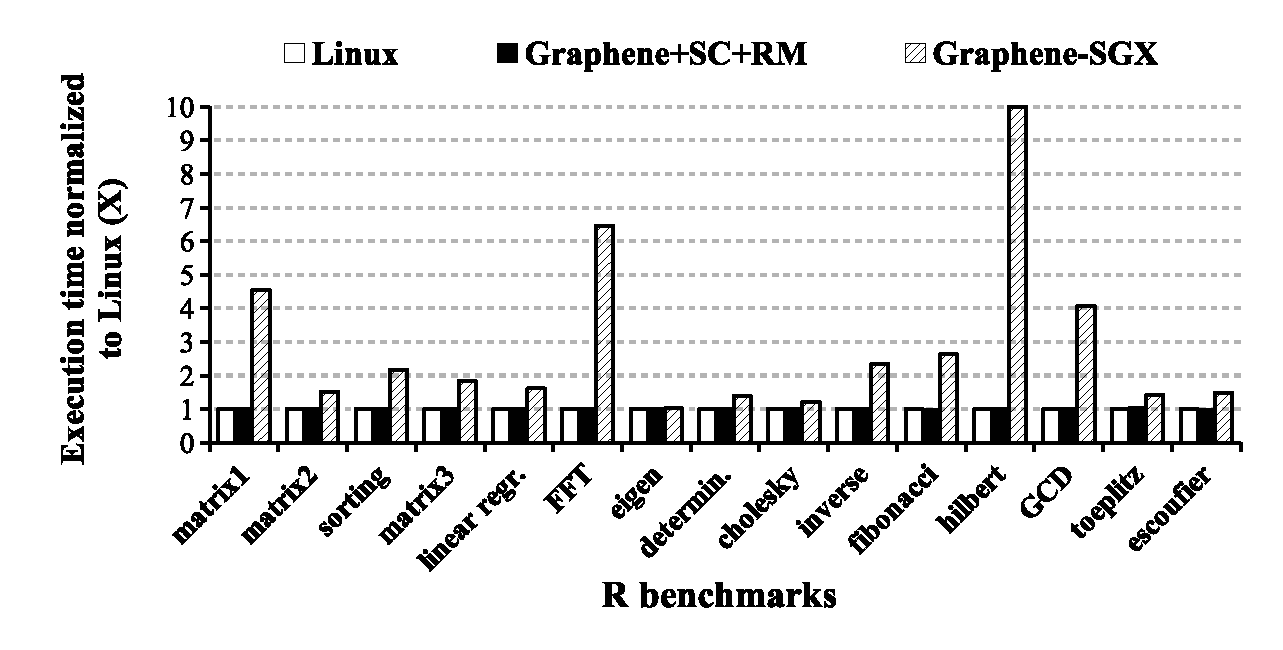
\includegraphics[width=38em]{r-overhead}\\
\caption{Performance overhead on desktop applications, including latency of R, execution time of GCC compilation, download time with CURL. The evaluation compares native Linux, \graphene{}, and \graphenesgx{}.} %{\bf Enclave creation time is deducted from the GCC execution time.}}
\label{fig:eval:r-overheads}
\end{figure}


\begin{figure}[t!]
\centering
\footnotesize
\begin{minipage}{.49\textwidth}
\centering
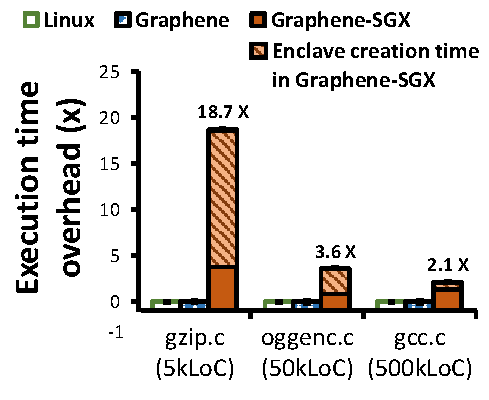
\includegraphics[width=20em]{sgx/gcc-overhead}\\
\vspace{3pt}
{\bf (b) GCC}
\end{minipage}
\begin{minipage}{.49\textwidth}
\centering
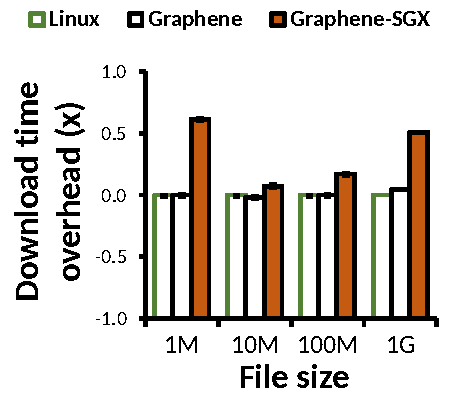
\includegraphics[width=20em]{sgx/curl-overhead}\\
\vspace{3pt}
{\bf (c) CURL}
\end{minipage}
\caption{Performance overhead on desktop applications, including latency of R, execution time of GCC compilation, download time with CURL. The evaluation compares native Linux, \graphene{}, and \graphenesgx{}.} %{\bf Enclave creation time is deducted from the GCC execution time.}}
\label{fig:desktop-overhead}
\end{figure}



\paragraph{Command-line applications}


We also evaluate the performance of a few commonly-used command-line applications.
%, to evaluate the performance of \graphenesgx{} on PCs instead of servers and clouds.
Three off-the-shelf applications are tested in our experiments:
{\bf R} (v3.2.3) for statistical computing~\cite{r-project}; {\bf GCC} (v5.4), the general GNU C compiler~\cite{gcc}; {\bf CURL} (v7.74), the default command-line web client on UNIX~\cite{curl}.
These applications are chosen because they are frequently used by Linux users,
and each of them potentially  be used 
in an enclave to handle sensitive data---either on a server or a client
machine.
% can realize profitable scenarios of using enclaves on desktop machines.



We evaluate the latency or execution time of these applications. 
%, because desktop users tend to care more about responsiveness than throughput.
In our experiments, both R and CURL have internal timing features to measure the wall time
of individual operations or executions.
%However, for other applications like GCC which does not include internal timing, evaluating the execution time can be influenced by many factors.
On a Linux host, the time to start a library OS is higher than a simple 
process, but significantly lower than booting a guest OS in a VM or
starting a container. 
Prior work measured Graphene (non-SGX) start time at 641 $\mu$s~\cite{tsai14graphene}, whereas starting an empty Linux VM takes 10.3s and starting a Linux (LXC) container takes 200 ms~\cite{agarwal15container}. 
%% dp; Note that this is MILLI seconds, not micro seconds.
%average memory footprint of an empty Linux VM, with memory deduplication, is about 96MB, . 


On SGX, the enclave creation time is relatively higher, \fixme{added more detailed number} ranging from 0.5s (a 256MB enclave) to 5s (a 2G enclave), which is a fixed cost that any application framework
will have to pay to run on SGX.
%For library OSes, the time for creating and initializing an enclave is not trivial, because it is similar to booting an lightweight OS.
% a significant part of the start-up time
% of an application is more significant, because creating enclaves is expensive.
%We consider the enclave creation time as a fixed cost for any application running in \graphenesgx{},
%and acceptable to users as long as it is responsive.
Enclave creation time is determined by the latency of the hardware and the Intel kernel driver, and is primarily a function of the size of 
the enclave, which is specified at creation time because it affects the enclave signature. %\fixmedp{although can't it grow with eadd?}.  
For non-server workloads that create multiple processes during execution,
such as GCC in Figure~\ref{fig:desktop-overhead},
the enclave creation contributes a significant portion to the execution time overheads, illustrated as a stacked bar.
%Since the enclave creation time is related to the enclave size, and unrelated to the workload,
%we deduct the enclave creation time from the execution time of GCC in Figure~\ref{fig:desktop-overhead}. \fixmedp{I think it might be better to show this as a stacked bar instead of just removing it.  Opaquely subtracting this cost doesn't seem right.  Let's discuss dp: I thought we agreed to change this...}

{\bf R}~\cite{r-project} is a scripting language often used for
data processing and statistical computation.
With enclaves, users can process sensitive data on an
OS they don't trust.
We use an R benchmark suite developed by Urbanek et al.~\cite{r-benchmark-25}, which includes 15 CPU-bound workloads such as matrix computation and number processing.
\graphenesgx{} slows down by less than 100\% on the majority of the workloads, excepts the ones which involve allocation and garbage collection: ({\tt matrix1} creates and destroys matrices, and both {\tt FFT} and {\tt hilbert} involve heavy garbage collection.)
Aside from garbage collection, these R benchmarks do not frequently interact with the host.
We further note that non-SGX \graphene{} is as efficient as Linux on all workloads, 
and these overheads appear to be SGX-specific.
%\fixmedp{Check this pontification}
In our experience, garbage collection and memory management code in managed language runtime
systems tends to be written with assumptions that do not match enclaves,
such as a large, sparse address space or that memory can be demand paged 
nearly for free (SGX version 1 requires all memory to be mapped
at creation); a useful area for future work would be to design
garbage collection strategies that are optimized for enclaves.
%we believe the overheads on \graphenesgx{} are contributed by enclaves.

{\bf GCC}~\cite{gcc} is a widely-used C compiler.
By supporting GCC in enclaves, developers can compile closed-source applications on customers' machines,
without leaking the source code.
GCC composes of multiple binaries, including {\tt cc1} (compiler), {\tt as} (assembler), and {\tt ld} (linker).
Therefore, GCC is a multi-process program using \syscall{execve}.
We test the compilation of thee source files with varied sizes,
using single C source files collected by MIT~\cite{gcc-benchmark}.
Each GCC execution typically \fixme{it's five, not four} creates five processes, and we run each process in a 256MB enclave by default.
%and has a fixed cost on enclave creation, which is unrelated to workload and depends on the enclave size.
%\fixme{check this}
\fixme{clarified this part, to prevent confusion between latency and overhead. also, GCC numbers got better.}
For a small workload like compiling {\tt gzip.c} (5 kLoC), running in \graphenesgx{} (4.1s) is 18.7$\times$ slower than Linux (0.2s).
The bulk of this time is spent in enclave creation, taking 3.0s in total, while the whole execution inside the enclaves, including initialization of the library OS and OS shield, takes only 1.1s, or 4.2$\times$ overhead.
For larger workloads like {\tt oggenc.c} (50 kLoC) and {\tt gcc.c} (500 kLoC), 
the overhead of \graphenesgx{} is less significant. % (3.6$\times$ and 2.1$\times$ overhead, respectively).
For {\tt gcc.c} (500 kLoC), we have to enlarge one of the enclaves ({\tt cc1}) to 2GB,
but running on \graphenesgx{} (53.1s) is only 2.1$\times$ slower than Linux (17.2s),
and 7.1s is spent on enclave creation.
%and the creation of four enclaves takes 8s.
%Each compilation has a fixed enclave creation time in \graphenesgx{}, which is about 1--2 seconds per enclave. We deduct the creation time of all enclaves  to gain more meaningful results, but do not hide rest of the overhead on fork.
%\fixmedp{Also not comfortable with this; add a bar?}
%In general, GCC in \graphenesgx{} is 1--5$\times$ slower than GCC on native Linux. 
%\fixmedp{This really needs some profiling if possible}
The overhead of non-SGX \graphene{} on GCC is marginal.




{\bf CURL}~\cite{curl} is a command-line  web downloader.
\graphenesgx{} can make CURL into a secure downloader that attests both server and client ends.
We evaluate the total time to download a large file, ranging from 1MB to 1GB, from another machine running Apache. % over Gigabit LAN.
%across high-speed university network\fixmedp{more specific, as above}.
\graphene{} has marginal overhead on CURL, and
\graphenesgx{} adds 7--61\% overhead to the downloading time of CURL, due to the latency of I/O.


\makeatletter
\def\input@path{{eval/}}
\makeatother
\graphicspath{{eval/figures/}}

